\documentclass{mimosis}

\usepackage{metalogo}

%%%%%%%%%%%%%%%%%%%%%%%%%%%%%%%%%%%%%%%%%%%%%%%%%%%%%%%%%%%%%%%%%%%%%%%%
% Some of my favourite personal adjustments
%%%%%%%%%%%%%%%%%%%%%%%%%%%%%%%%%%%%%%%%%%%%%%%%%%%%%%%%%%%%%%%%%%%%%%%%
%
% These are the adjustments that I consider necessary for typesetting
% a nice thesis. However, they are *not* included in the template, as
% I do not want to force you to use them.

% This ensures that I am able to typeset bold font in table while still aligning the numbers
% correctly.
\usepackage{etoolbox}

%%%%%%%%%%%%%%%%%%%%%%%%%%%%%%%%%%%%%%%%%%%%%%%%%%%%%%%%%%%%%%%%%%%%%%%%
% Hyperlinks & bookmarks
%%%%%%%%%%%%%%%%%%%%%%%%%%%%%%%%%%%%%%%%%%%%%%%%%%%%%%%%%%%%%%%%%%%%%%%%

\usepackage[%
  colorlinks = true,
  citecolor  = RoyalBlue,
  linkcolor  = RoyalBlue,
  urlcolor   = RoyalBlue,
  unicode,
  ]{hyperref}

\usepackage{bookmark}

\usepackage{algorithm}
\usepackage{algpseudocode}

%%%%%%%%%%%%%%%%%%%%%%%%%%%%%%%%%%%%%%%%%%%%%%%%%%%%%%%%%%%%%%%%%%%%%%%%
% Bibliography
%%%%%%%%%%%%%%%%%%%%%%%%%%%%%%%%%%%%%%%%%%%%%%%%%%%%%%%%%%%%%%%%%%%%%%%%
%
% I like the bibliography to be extremely plain, showing only a numeric
% identifier and citing everything in simple brackets. The first names,
% if present, will be initialized. DOIs and URLs will be preserved.

\usepackage[%
  autocite     = plain,
  backend      = biber,
  doi          = true,
  url          = true,
  giveninits   = true,
  hyperref     = true,
  maxbibnames  = 99,
  maxcitenames = 99,
  sortcites    = true,
  style        = numeric,
  ]{biblatex}

%%%%%%%%%%%%%%%%%%%%%%%%%%%%%%%%%%%%%%%%%%%%%%%%%%%%%%%%%%%%%%%%%%%%%%%%
% Some adjustments to make the bibliography more clean
%%%%%%%%%%%%%%%%%%%%%%%%%%%%%%%%%%%%%%%%%%%%%%%%%%%%%%%%%%%%%%%%%%%%%%%%
%
% The subsequent commands do the following:
%  - Removing the month field from the bibliography
%  - Fixing the Oxford commma
%  - Suppress the "in" for journal articles
%  - Remove the parentheses of the year in an article
%  - Delimit volume and issue of an article by a colon ":" instead of
%    a dot ""
%  - Use commas to separate the location of publishers from their name
%  - Remove the abbreviation for technical reports
%  - Display the label of bibliographic entries without brackets in the
%    bibliography
%  - Ensure that DOIs are followed by a non-breakable space
%  - Use hair spaces between initials of authors
%  - Make the font size of citations smaller
%  - Fixing ordinal numbers (1st, 2nd, 3rd, and so) on by using
%    superscripts

% Remove the month field from the bibliography. It does not serve a good
% purpose, I guess. And often, it cannot be used because the journals
% have some crazy issue policies.
\AtEveryBibitem{\clearfield{month}}
\AtEveryCitekey{\clearfield{month}}

% Fixing the Oxford comma. Not sure whether this is the proper solution.
% More information is available under [1] and [2].
%
% [1] http://tex.stackexchange.com/questions/97712/biblatex-apa-style-is-missing-a-comma-in-the-references-why
% [2] http://tex.stackexchange.com/questions/44048/use-et-al-in-biblatex-custom-style
%
\AtBeginBibliography{%
  \renewcommand*{\finalnamedelim}{%
    \ifthenelse{\value{listcount} > 2}{%
      \addcomma
      \addspace
      \bibstring{and}%
    }{%
      \addspace
      \bibstring{and}%
    }
  }
}

% Suppress "in" for journal articles. This is unnecessary in my opinion
% because the journal title is typeset in italics anyway.
\renewbibmacro{in:}{%
  \ifentrytype{article}
  {%
  }%
  % else
  {%
    \printtext{\bibstring{in}\intitlepunct}%
  }%
}

% Remove the parentheses for the year in an article. This removes a lot
% of undesired parentheses in the bibliography, thereby improving the
% readability. Moreover, it makes the look of the bibliography more
% consistent.
\renewbibmacro*{issue+date}{%
  \setunit{\addcomma\space}
    \iffieldundef{issue}
      {\usebibmacro{date}}
      {\printfield{issue}%
       \setunit*{\addspace}%
       \usebibmacro{date}}%
  \newunit}

% Delimit the volume and the number of an article by a colon instead of
% by a dot, which I consider to be more readable.
\renewbibmacro*{volume+number+eid}{%
  \printfield{volume}%
  \setunit*{\addcolon}%
  \printfield{number}%
  \setunit{\addcomma\space}%
  \printfield{eid}%
}

% Do not use a colon for the publisher location. Instead, connect
% publisher, location, and date via commas.
\renewbibmacro*{publisher+location+date}{%
  \printlist{publisher}%
  \setunit*{\addcomma\space}%
  \printlist{location}%
  \setunit*{\addcomma\space}%
  \usebibmacro{date}%
  \newunit%
}

% Ditto for other entry types.
\renewbibmacro*{organization+location+date}{%
  \printlist{location}%
  \setunit*{\addcomma\space}%
  \printlist{organization}%
  \setunit*{\addcomma\space}%
  \usebibmacro{date}%
  \newunit%
}

% Display the label of a bibliographic entry in bare style, without any
% brackets. I like this more than the default.
%
% Note that this is *really* the proper and official way of doing this.
\DeclareFieldFormat{labelnumberwidth}{#1\adddot}

% Ensure that DOIs are followed by a non-breakable space.
\DeclareFieldFormat{doi}{%
  \mkbibacro{DOI}\addcolon\addnbspace
    \ifhyperref
      {\href{http://dx.doi.org/#1}{\nolinkurl{#1}}}
      %
      {\nolinkurl{#1}}
}

% Use proper hair spaces between initials as suggested by Bringhurst and
% others.
\renewcommand*\bibinitdelim {\addnbthinspace}
\renewcommand*\bibnamedelima{\addnbthinspace}
\renewcommand*\bibnamedelimb{\addnbthinspace}
\renewcommand*\bibnamedelimi{\addnbthinspace}

% Make the font size of citations smaller. Depending on your selected
% font, you might not need this.
\renewcommand*{\citesetup}{%
  \biburlsetup
  \small
}

\DeclareLanguageMapping{english}{english-mimosis}

% Make hyperlinks extend to the author name if `\textcite` is being used
% instead of another cite command.

\DeclareFieldFormat{citehyperref}{%
  % Need this to avoid nested links
  \DeclareFieldAlias{bibhyperref}{noformat}%
  \bibhyperref{#1}%
}

\DeclareFieldFormat{textcitehyperref}{%
  % Need this to avoid nested links
  \DeclareFieldAlias{bibhyperref}{noformat}%
  \bibhyperref{%
    #1%
    \ifbool{cbx:parens}
      {\bibcloseparen\global\boolfalse{cbx:parens}}
      {}%
    }%
}

\savebibmacro{cite}
\savebibmacro{textcite}

\renewbibmacro*{cite}{%
  \printtext[citehyperref]{%
    \restorebibmacro{cite}%
    \usebibmacro{cite}}%
}

\renewbibmacro*{textcite}{%
  \ifboolexpr{
    ( not test {\iffieldundef{prenote}} and
      test {\ifnumequal{\value{citecount}}{1}} )
    or
    ( not test {\iffieldundef{postnote}} and
      test {\ifnumequal{\value{citecount}}{\value{citetotal}}} )
  }%
  {\DeclareFieldAlias{textcitehyperref}{noformat}}
  {}%
  \printtext[textcitehyperref]{%
    \restorebibmacro{textcite}%
    \usebibmacro{textcite}}%
}

\addbibresource{Thesis.bib}

%%%%%%%%%%%%%%%%%%%%%%%%%%%%%%%%%%%%%%%%%%%%%%%%%%%%%%%%%%%%%%%%%%%%%%%%
% Fonts
%%%%%%%%%%%%%%%%%%%%%%%%%%%%%%%%%%%%%%%%%%%%%%%%%%%%%%%%%%%%%%%%%%%%%%%%

\ifxetexorluatex
  \usepackage{unicode-math}
  \setmainfont{EB Garamond}
  \setmathfont{Garamond Math}
  \setmonofont[Scale=MatchLowercase]{Source Code Pro}
\else
  \usepackage[lf]{ebgaramond}
  % \usepackage[default]{raleway}
  \usepackage[oldstyle,scale=0.7]{sourcecodepro}
  \singlespacing
\fi

\newacronym{GNN}{GNN}{Graph Neural Network}
\newacronym{SOTA}{SOTA}{State-of-the-art}

\newglossaryentry{LaTeX}{%
  name        = {\LaTeX},
  description = {A document preparation system},
  sort        = {LaTeX},
}

\newglossaryentry{Real numbers}{%
  name        = {$\real$},
  description = {The set of real numbers},
  sort        = {Real numbers},
}

\makeindex
\makeglossaries

%%%%%%%%%%%%%%%%%%%%%%%%%%%%%%%%%%%%%%%%%%%%%%%%%%%%%%%%%%%%%%%%%%%%%%%%
% Ordinals
%%%%%%%%%%%%%%%%%%%%%%%%%%%%%%%%%%%%%%%%%%%%%%%%%%%%%%%%%%%%%%%%%%%%%%%%

\makeatletter
\@ifundefined{st}{%
  \newcommand{\st}{\textsuperscript{\textup{st}}\xspace}
}{}
\@ifundefined{rd}{%
  \newcommand{\rd}{\textsuperscript{\textup{rd}}\xspace}
}{}
\@ifundefined{nd}{%
  \newcommand{\nd}{\textsuperscript{\textup{nd}}\xspace}
}{}
\makeatother

\renewcommand{\th}{\textsuperscript{\textup{th}}\xspace}

%%%%%%%%%%%%%%%%%%%%%%%%%%%%%%%%%%%%%%%%%%%%%%%%%%%%%%%%%%%%%%%%%%%%%%%%
% Incipit
%%%%%%%%%%%%%%%%%%%%%%%%%%%%%%%%%%%%%%%%%%%%%%%%%%%%%%%%%%%%%%%%%%%%%%%%

\title{Accelerating GNN Inference with Dynamic GPU Feature Caches}
% \subtitle{Undergraduate Honors Thesis}
\author{Henry Liu \\ \texttt{henry.liu@utexas.edu}}

\begin{document}

\frontmatter
  \begin{titlepage}
  \vspace*{5cm}
  \makeatletter
  \begin{center}
    \begin{Huge}
      \@title
    \end{Huge}\\
    % [0.1cm]
    %
    \begin{Large}
      \@subtitle
    \end{Large}
    %
    \emph{by}\\
    \begin{Large}
        \@author\\
    \end{Large}
    \begin{Large}
        \vspace{5mm}
        Advised by Dr. Aditya Akella
    \end{Large}
    %
    \vfill
    A document submitted in partial fulfillment
    of the requirements for the degree of\\
    \emph{Technical Report}\\
    at\\
    \textsc{University of Texas at Austin}
  \end{center}
  \makeatother
\end{titlepage}

% \newpage
% \null
% \thispagestyle{empty}
% \newpage

  \begin{center}
  \textsc{Abstract}
\end{center}
%
\noindent
%

Graph Neural Networks (GNNs) have gained significant popularity due to their excellent performance in many graph representation learning tasks. 
Graphs used for GNN computation usually associate high-dimensional feature vectors with each node, which must be copied to the GPU for GNN execution.
This work investigates how GNN inference systems can dynamically cache graph features in GPU memory to reduce request-response latencies.
% can respond to inference requests quickly without compromising prediction accuracy.

Existing GNN literature has identified that efficiently moving graph features to GPUs, known as data loading, is an important challenge at training time. 
To reduce data loading overheads, state of the art GNN training systems statically cache graph features on the GPU.
We observe that the data loading problem is exacerbated at inference time and becomes a disproportionate bottleneck when serving inference requests. We improve upon existing static caching techniques to be better suited for inference. 

In particular, we motivate the use of dynamic cache policies to exploit graph locality of inference requests and explore mechanisms to reduce the impact of dynamic cache overheads on latency and throughput. 
Our system targets a single-machine, multi-GPU setting and performs cache updates asynchronously to remove cache update operations from the latency-sensitive request-response path.
We show how a simple frequency-based cache admission and eviction policy can achieve better cache hit rates than existing static cache baselines.
We then leverage interconnects such as NVLink to allow multiple GPUs to share a single logical cache and propose a lock-free synchronization mechanism to reduce lock contention due to cache updates. 

  \tableofcontents

\mainmatter

  % \part[A good part]{%
  %   A good part\\
  %   %
  %   \vspace{1cm}
  %   %
  %   \begin{minipage}[l]{\textwidth}
  %   %
  %   \textnormal{%
  %     \normalsize
  %     %
  %     \begin{singlespace*}
  %       \onehalfspacing
  %       %
  %       You can also use parts in order to partition your great work
  %       into larger `chunks'. This involves some manual adjustments in
  %       terms of the layout, though.
  %     \end{singlespace*}
  %   }
  %   \end{minipage}
  % }

  %%%%%%%%%%%%%%%%%%%%%%%%%%%%%%%%%%%%%%%%%%%%%%%%%%%%%%%%%%%%%%%%%%%%%%%%
\chapter{Introduction}
%%%%%%%%%%%%%%%%%%%%%%%%%%%%%%%%%%%%%%%%%%%%%%%%%%%%%%%%%%%%%%%%%%%%%%%%

% \begin{center}
%   \begin{minipage}{0.5\textwidth}
%     \begin{small}
%       In which the reasons for creating this package are laid bare for the
%       whole world to see and we encounter some usage guidelines.
%     \end{small}
%   \end{minipage}
%   \vspace{0.5cm}
% \end{center}

Graphs are increasingly popular and highly expressive structures for representing data.
In the past decade, significant interest in graph analysis has led to the emergence of Graph Neural Networks (GNNs), class of state-of-the-art machine learning methods for graph representation learning. 

GNNs adopt ideas from traditional Deep Neural Networks (DNNs) and combine them with techniques to capture structural information about graphs. Traditional DNNs have excelled in various tasks in areas such as computer vision \cite{AlexNet_2012}\cite{YOLO_2016} and natural language processing \cite{RNN_2013}\cite{NamedEntityRecognition_2016}. In these domains, however, inputs exhibit fairly regular structure, unlike in graphs. 

To bridge the gap between DNNs and graph-structured data, GNNs capture graph structural information by using graph \textit{convolutions}, a technique for aggregating local node neighborhood information. As opposed to traditional graph processing, graphs used with GNNs associate \textit{features} with each node in the graph, which are large multidimensional tensors. GNNs use these features to compute \textit{embeddings} for each node in the graph by recursively aggregating each node's neighboring features. 
The resulting embeddings can be used for tasks such as node classification, link prediction, or graph classification.

% Different GNN architectures such as Graph Convolutional Networks (GCN) \cite{GCN_2016}, GraphSAGE \cite{GraphSAGE_2017}, and Graph Attention Networks (GAT) \cite{GAT_2018} perform different types of aggregations and operations on features, but share the same neighborhood aggregation principle.


GNNs are deployed in production systems for many applications, including bioinformatics \cite{Bioinfo_2021} \cite{Bioinfo_2022}, 
traffic forecasting \cite{Traffic_SST-GNN_2021} \cite{Traffic_GoogleMaps_2021} \cite{Traffic_survey_2021}, recommendation systems \cite{Recsys_PinSAGE_2018} \cite{Recsys_Diffnet_2022}\cite{Recsys_LightGCN_2020}\cite{Recsys_NAGCN_2020}\cite{Recsys_SGL_2021}\cite{Recsys_Survey_2022}, 
cybersecurity \cite{Cybersec_2022} \cite{Cybersec_2023}, and combinatorial optimization \cite{CombinatorialOptimization_2019}\cite{CombinatorialOptimization_2021}, among many others. Although there has been significant work on GNN training systems [todo cite stuff], GNN inference is relatively understudied. 

Many existing GNN inference systems rely on approximate nearest neighbor approaches or periodic offline inference to keep node embeddings fresh \cite{Recsys_PinSAGE_2018} \cite{Recsys_Survey_2022}. However, such approaches may not meet accuracy, latency, or throughput demands of real world systems. For example, in 2013 Facebook's graph database was updated roughly eight-six thousand times per second \cite{Graph_Survey_2020}.

% Thus in this work we look at creating an efficient system for online GNN inference. 
To understand the current state of the art for online GNN inference, we first examine how key optimizations in GNN training systems can apply to GNN inference. One critical optimization we identify is node \textit{feature caching}, the act of storing some node features in GPU memory to avoid redundant host-device transfers.
However, only some caching techniques from GNN training systems are applicable at inference time.
The simplest of these is static degree-based caching, which permanently places features corresponding to nodes with highest out-degree in GPU memory \cite{PaGraph_2020}.
We observe that even when using this static cache, GNN inference still encounters the \textit{data loading} bottleneck, where 30-80\% of inference latency is due to copying node features to the GPU.
Although improving cache hit rate would help alleviate this bottleneck, no GNN training systems implement dynamic caches, even using traditional LRU or LFU cache eviction policies, due to the associated overhead.

We tackle the challenges associated with efficiently implementing dynamic caches in three ways.

First, we motivate the use of dynamic cache policies by noting that GNN inference requests create opportunities to exploit graph locality not present at training time. Assuming mini-batch training, GNNs are trained mini-batches that are generally sampled uniformly randomly from the entire graph. However, at inference time, GNNs need to produce answers for new requests that connect into the existing graph. These requests can exhibit locality in graph structure due to factors such as user trends, leading to "hot" subgraphs.

We then propose a simple frequency-based admission and eviction policy provides better cache hit rates than static caches or traditional policies such as LFU. We demonstrate that this holds across inferences traces corresponding to uniformly sampled requests as well as requests concentrated in hot subgraphs.

Second, we use asynchrony as a technique to avoid overheads due to dynamic cache updates. Although dynamic caches can provide better cache hit rates, end-to-end performance can be eroded due to the overhead of actually performing cache updates. By moving cache update operations to separate host threads and CUDA streams, we take these operations off of the critical path when responding to inference requests. 

Lastly, we propose a lock-free mechanism for performing cache updates. In a system with many inference threads and pipelining, an asynchronous cache update can produce end-to-end performance equivalent to that of a synchronous one if it blocks pipeline stages due to naive locking. Furthermore, our system supports sharing of a single logical cache among multiple GPUs connected by NVLink, and the blocking of inter-GPU communication can exacerbate locking overheads. To address this we show how the cache can be \textit{masked} to allow for wait-free readers and lock-free writers.

% %%%%%%%%%%%%%%%%%%%%%%%%%%%%%%%%%%%%%%%%%%%%%%%%%%%%%%%%%%%%%%%%%%%%%%%%
% \section{Contributions}
% %%%%%%%%%%%%%%%%%%%%%%%%%%%%%%%%%%%%%%%%%%%%%%%%%%%%%%%%%%%%%%%%%%%%%%%%
% In this work, we analyze the outsized impact of feature movement from CPU to GPU on GNN inference. 
% Even when using static caching techniques borrowed from GNN training, this data loading step still remains a major bottleneck in achieving low latency inference. Gathering features in host memory and copying to the GPU comprises roughly 50\%-80\% of end-to-end inference latency. We tackle this problem by improving GPU feature caches in the following ways.
  %%%%%%%%%%%%%%%%%%%%%%%%%%%%%%%%%%%%%%%%%%%%%%%%%%%%%%%%%%%%%%%%%%%%%%%%
\chapter{Background and Motivation}
%%%%%%%%%%%%%%%%%%%%%%%%%%%%%%%%%%%%%%%%%%%%%%%%%%%%%%%%%%%%%%%%%%%%%%%%

%%%%%%%%%%%%%%%%%%%%%%%%%%%%%%%%%%%%%%%%%%%%%%%%%%%%%%%%%%%%%%%%%%%%%%%%
\section{Graph Neural Networks}
%%%%%%%%%%%%%%%%%%%%%%%%%%%%%%%%%%%%%%%%%%%%%%%%%%%%%%%%%%%%%%%%%%%%%%%
Given a graph containing nodes, edges, and features, Graph Neural Networks (GNNs) output a per-node \textit{embedding} for each node in the graph.
An embedding is a $d$-dimensional representation of aggregated feature information from a node's neighborhood. 
Similarity in the embedding space has different meaning based on the learning task, such as similarity of node type (a node classification task) \cite{GCN_2016} or likelihood of edge existence (a link prediction task) \cite{LinkPredictionGNN_2018}. 

% In this work we will consider the case where graphs are homogeneous (one node type) and only nodes have associated features.

Borrowing notation from P3 \cite{P3_2021}, we can generally represent the embedding for a node $v$ at layer $k$ as $h_v^k$, where
\begin{align} \label{GNN Equation}
    h_v^k = \sigma \biggl(
         W^k \cdot 
         \mathtt{COMBINE}^{(k)} \left(
            h_v^{k-1},
            \mathtt{AGG}^{(k)} \left( 
                    \{ h_u^{k-1} \mid u \in N(v) \}
                \right) 
         \right)
     \biggl)
\end{align}
\begin{align*}
    \sigma &= \text{Nonlinear function} \\
    W^k &= \text{Trainable weight matrix for layer $k$} \\
    N(v) &= \text{Neighborhood of node v}
\end{align*}
$\mathtt{AGG}^{(k)}$ is a function that aggregates the previous layer embeddings of node $v$'s neighborhood. 
$\mathtt{COMBINE}^{(k)}$ is a function that combines the result of $\mathtt{AGG}^{(k)}$ with $v$'s own last layer embedding. 
The first layer embedding for node $v$, $h_k^0$, is just its original features.

The choice of $\mathtt{AGG}^{(k)}$ and $\mathtt{COMBINE}^{(k)}$ depend on the specific GNN architecture. Graph Convolutional Networks (GCN) \cite{GCN_2016}, GraphSAGE \cite{GraphSAGE_2017}, and Graph Attention Networks (GAT) \cite{GAT_2018} perform different types of aggregations and operations on features but share the same general aggregation principle.

Since for each layer there is a different $W^k$, GNNs are comprised of $k$ neural networks. Furthermore, each layer requires recursive computation on a node's neighbors. Thus a \textit{$k$-hop neighborhood} must be constructed to run a $k$-layer GNN.
Generally, GNNs use 1-5 layers, with 2 layers being a de facto standard \cite{Survey_First_2022}. However, some architectures can use significantly more layers, such as the current SOTA EnGCN model comprising 8 layers \cite{EnGCN_2023}.
Figure \ref{Background: GNN Execution Example} illustrates the construction of a \textit{computation graph} for a $2$-layer GNN. A computation graph describes how necessary nodes and edges participate in GNN computation.


\begin{figure}[h!]
    \begin{minipage}[c]{0.5\textwidth}
        \centering
        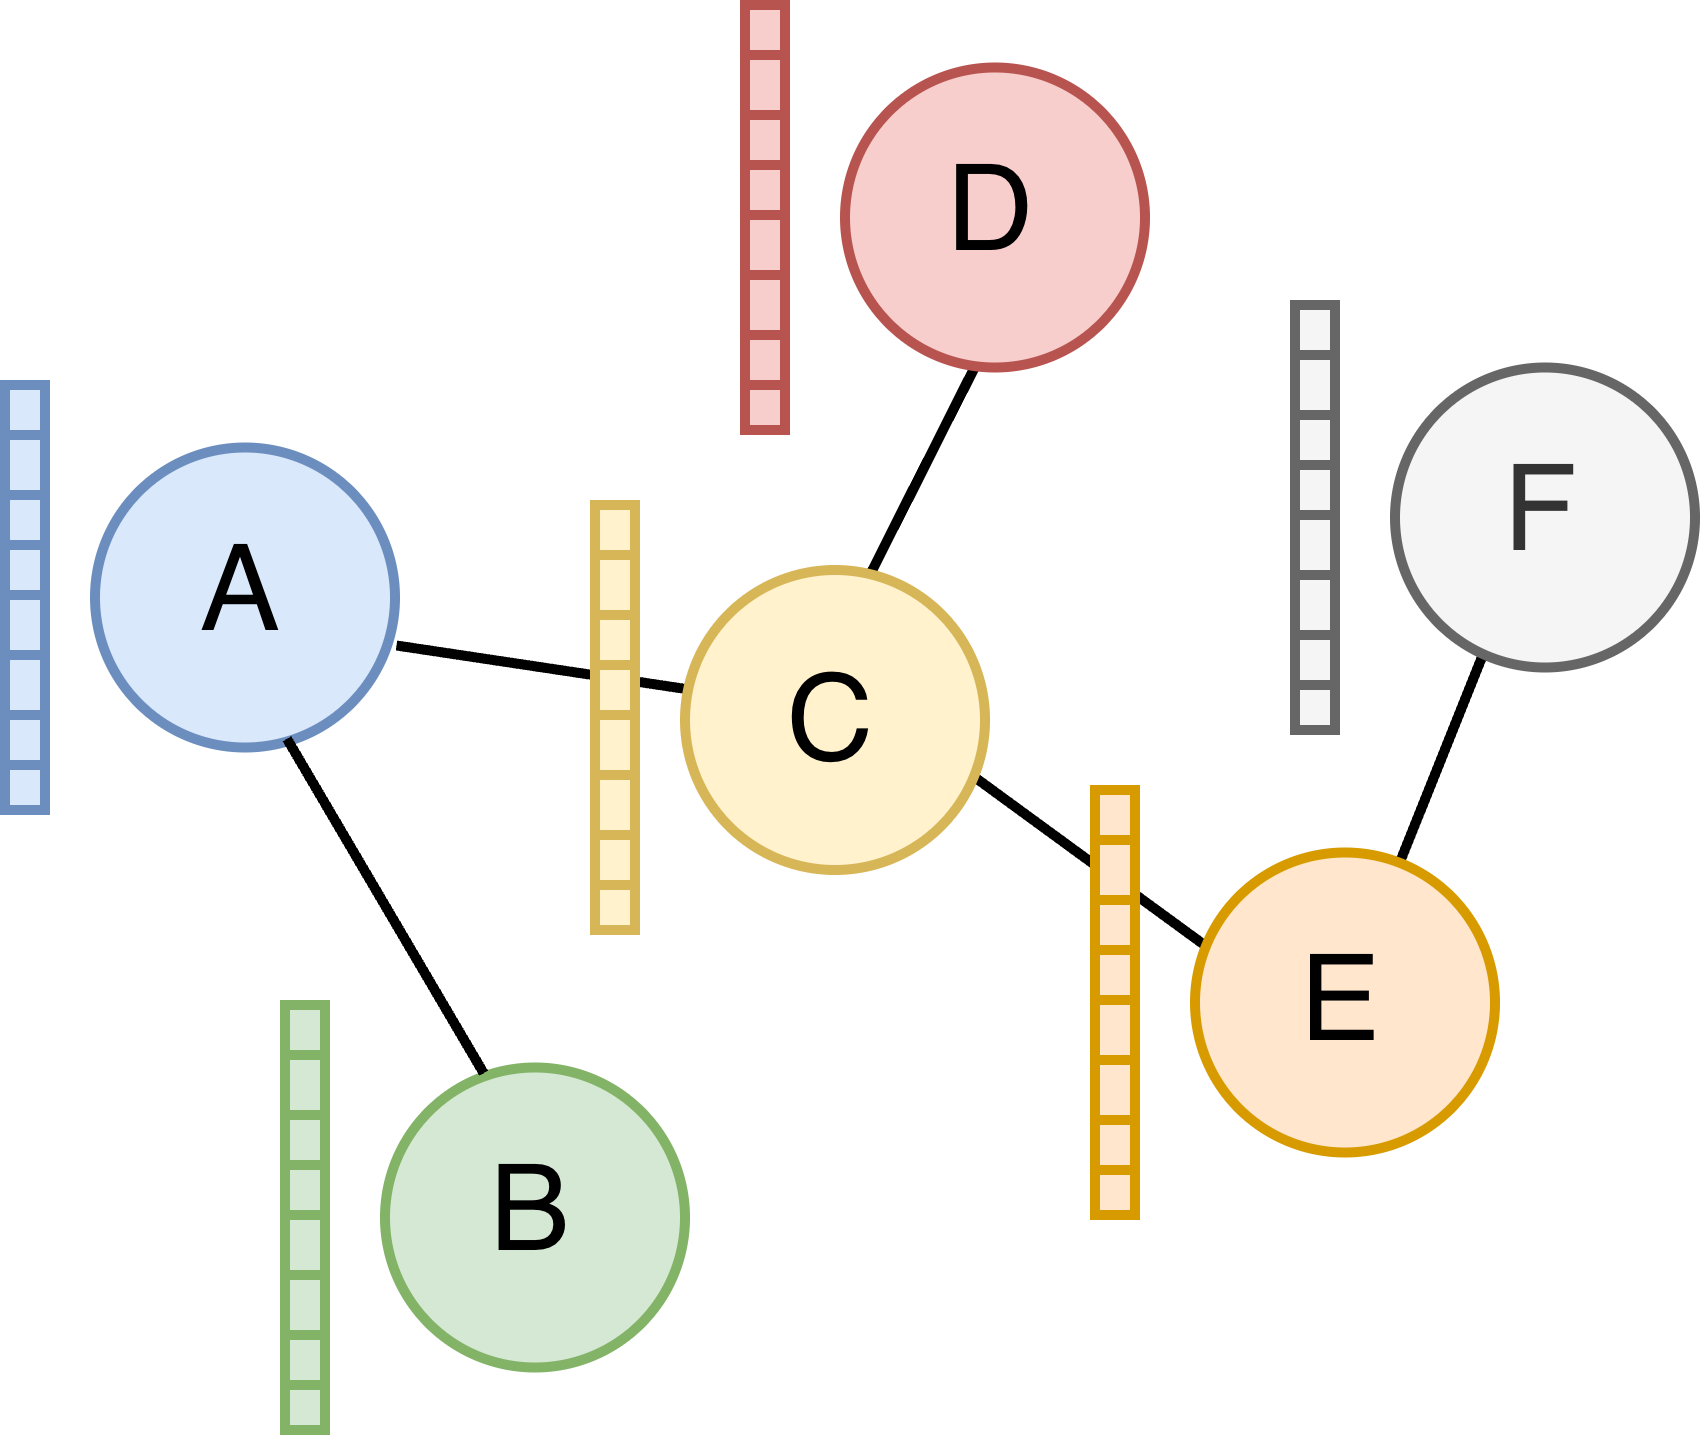
\includegraphics[width=0.85\textwidth]{diagrams/group_meeting_gnn-Graph structure.png}    
        % \caption{Graph structure and associated node features (colored bars).}
    \end{minipage}
    \hfill
    \begin{minipage}[c]{0.45\textwidth}
        \centering
        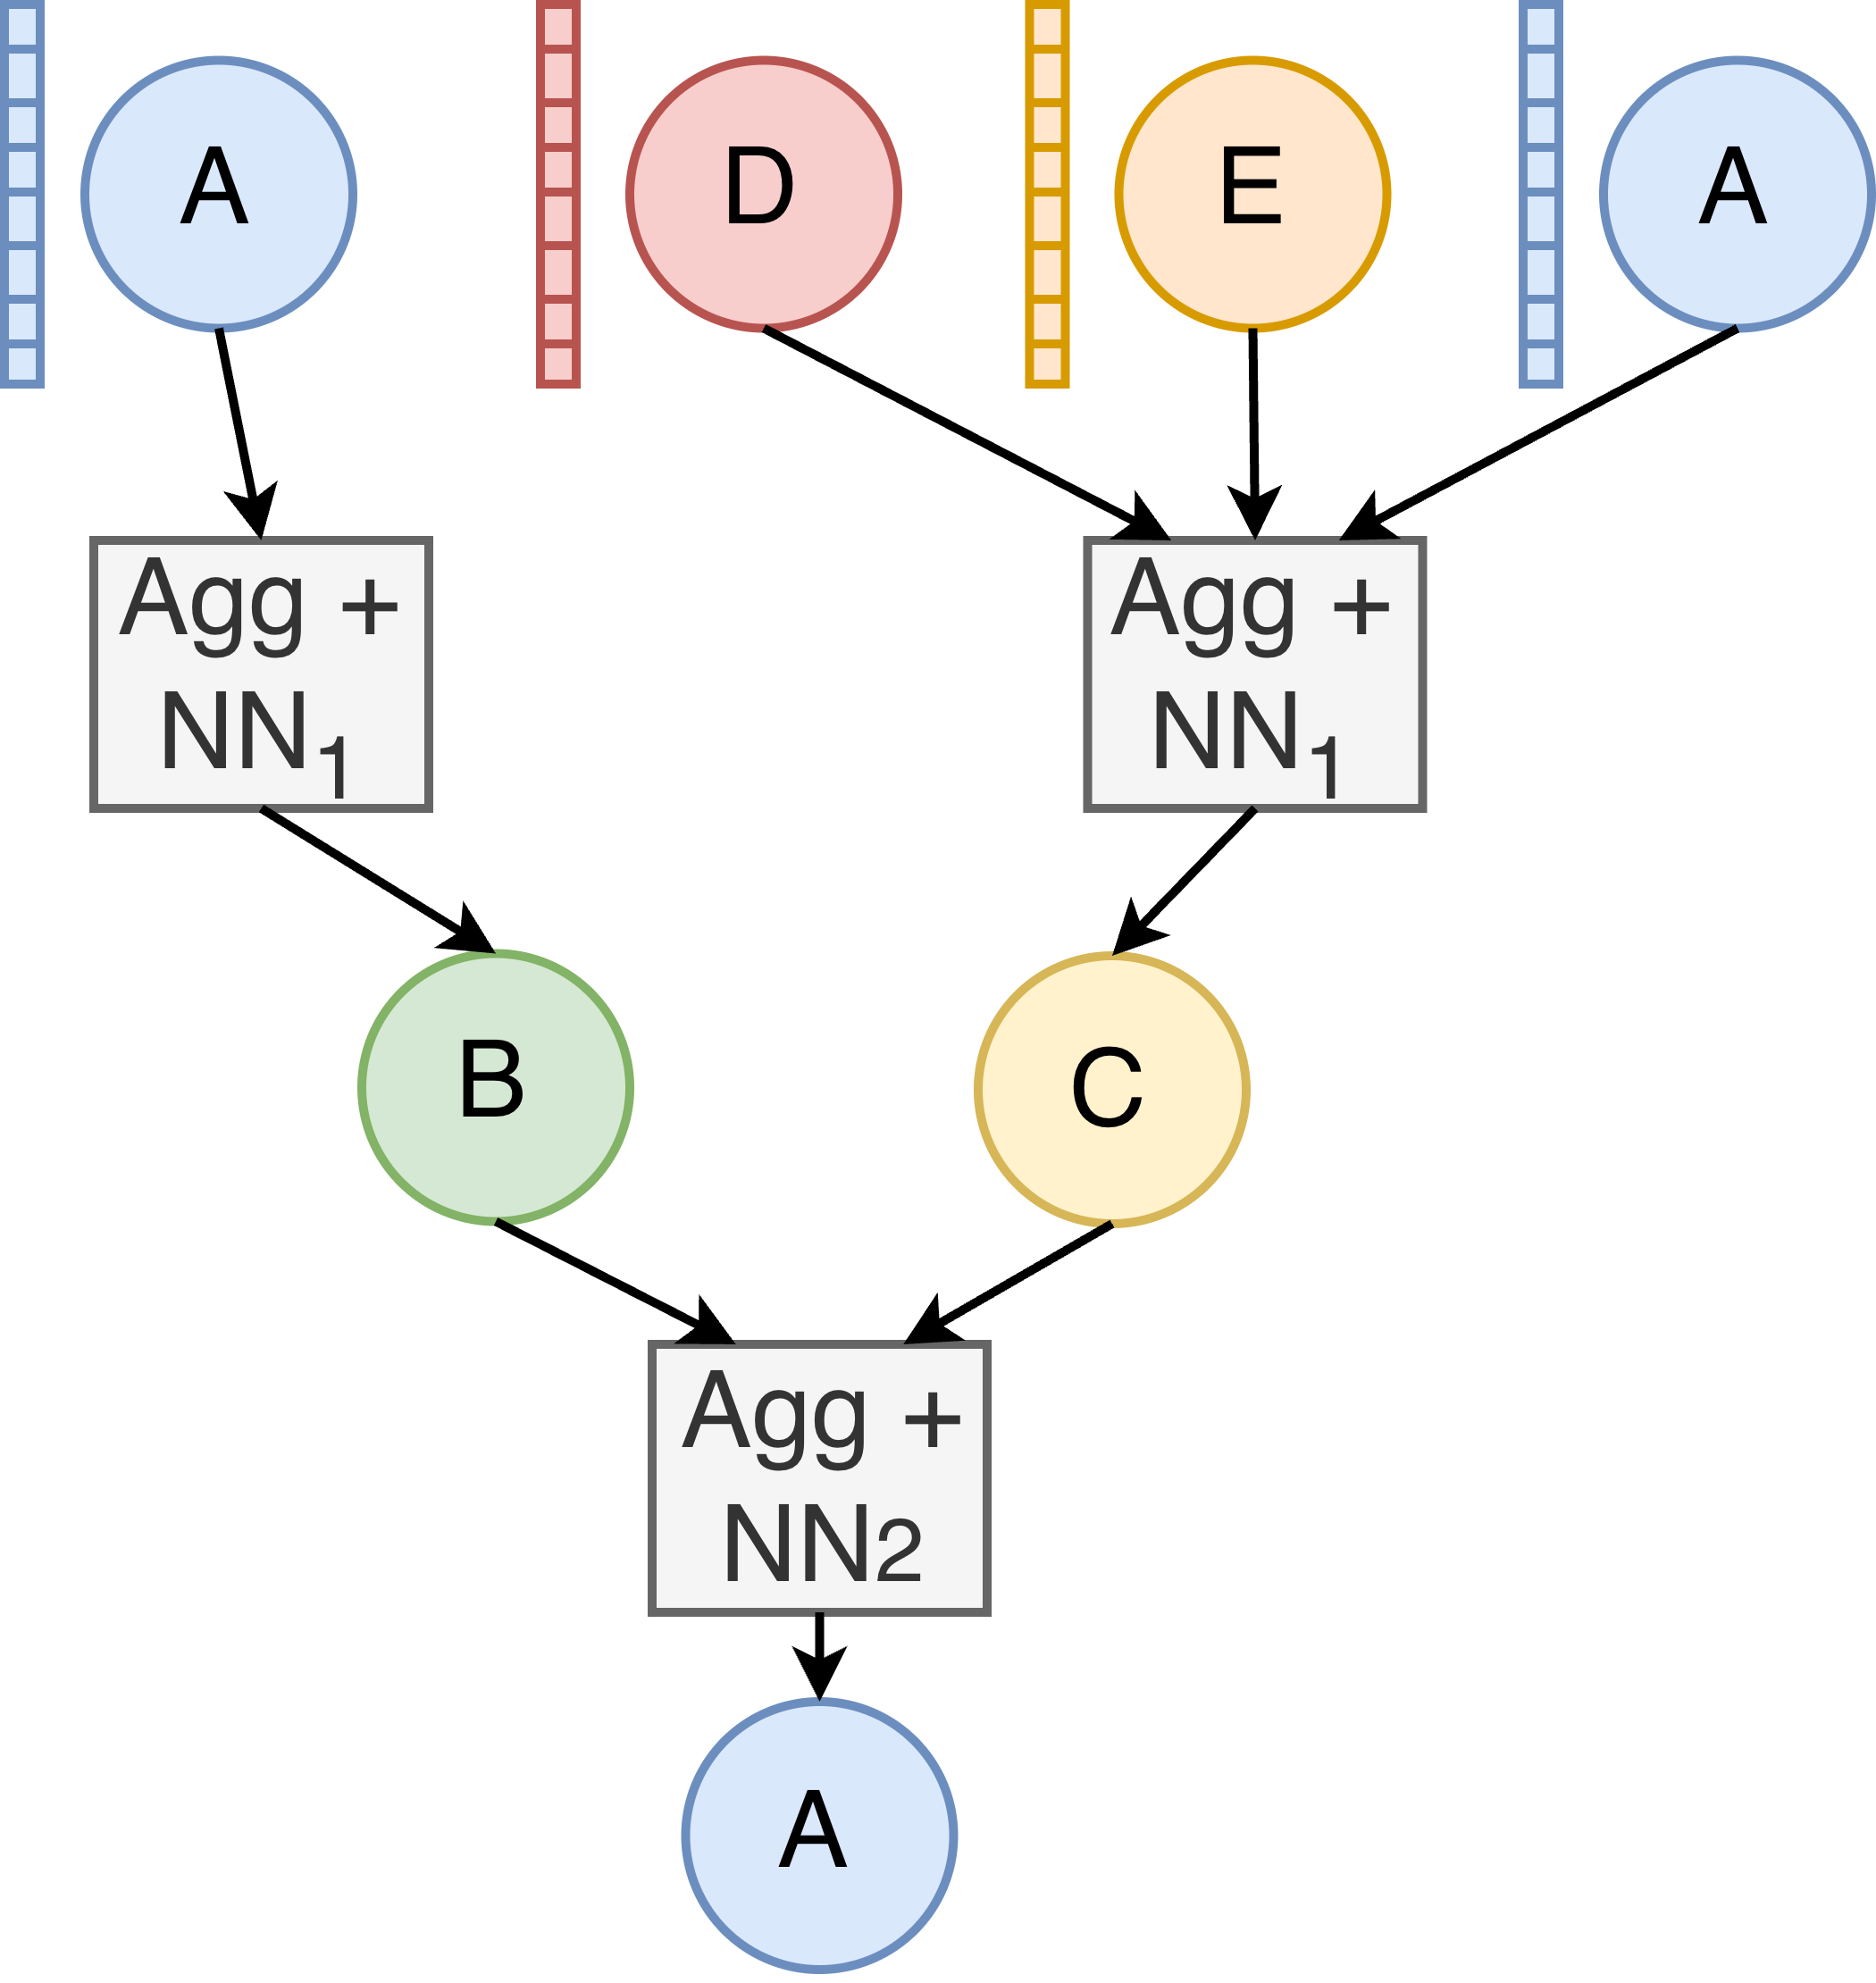
\includegraphics[width=0.95\textwidth]{diagrams/group_meeting_gnn-GNN Execution.png}
        % \caption{2-hop neighborhood and computation graph for node $A$, ignoring self loops.}
    \end{minipage}
    \caption{Graph and associated computation graph for node $A$.}
    \label{Background: GNN Execution Example}
\end{figure}    

%%%%%%%%%%%%%%%%%%%%%%%%%%%%%%%%%%%%%%%%%%%%%%%%%%%%%%%%%%%%%%%%%%%%%%%%
\section{Online GNN Inference}
%%%%%%%%%%%%%%%%%%%%%%%%%%%%%%%%%%%%%%%%%%%%%%%%%%%%%%%%%%%%%%%%%%%%%%%%
% [todo define what inference is?]
Traditionally, GNN inference has been viewed as an \textit{offline} problem, where inference is performed on all nodes in the graph (full graph inference).
Full graph inference is typically used for evaluating trained models or computing node embeddings for future lookups. 
For example, PinSage \cite{Recsys_PinSAGE_2018} first uses MapReduce \cite{MapReduce_2004} to perform full graph inference before storing all node embeddings in a database.
Then, PinSage uses $K$-nearest neighbors to compute embeddings for new queries, enabling it to serve online recommendation requests.
However, this approach, along with other nearest neighbor approaches, suffers from a loss in accuracy compared to directly using a GNN to compute the new embedding.

Therefore, in this work we will view GNN inference as an \textit{online} problem, where a GNN is given a request to compute an embedding for a node or batch of nodes. In this setting, requests consist of nodes, their features, and edges connecting them to the existing graph.

In this section we motivate this online inference formulation and present a concrete taxonomy of the stages of GNN inference.

\subsection{Online Inference Applications}
Online inference has many applications depending on domain.
For example, in a social network graph, an inference request can correspond to computing the embedding for a new user or recomputing embeddings as a result of a new friendship. 
Furthermore, there is no strict requirement that a node is truly "new", meaning that an inference request could correspond to an update of node features.
For example, in a traffic forecasting application, an inference request can be an update of node features that represent a change in traffic conditions.

% Facebook's social network graph in 2013 experienced roughly 86 thousand node or edge updates per second \cite{Graph_Survey_2020}. [todo put this in context]

\subsection{GNN Inference Stages}
While online GNN inference is generally understudied, it shares many similarities with GNN mini-batch training (discussed in Section \ref{Background: Relation to training}). Thus when understanding the steps required to perform GNN inference, we use established taxonomy from mini-batch training work \cite{PaGraph_2020}\cite{GNNLab_2022}\cite{P3_2021}. We break down the stages of GNN inference as follows:

\begin{enumerate}
    \item \textbf{Sampling:} Construct $k$-hop neighborhood for target nodes and build logical computation graph describing GNN computation.
    \item \textbf{Data Loading:} Moving necessary data to GPU, comprising two steps.
    \begin{enumerate}
        \item \textbf{Feature gather:} Gather node features corresponding to $k$-hop neighborhood in contiguous CPU buffer.
        \item \textbf{CPU-GPU copy:} Copy buffer with node features and computation graph to GPU.
    \end{enumerate}
    \item \textbf{Model execution:} Perform GNN computation on GPU.
\end{enumerate}
These stages are illustrated in Figure \ref{Compute Visualization}.

\begin{figure}[h!!!]
    \centering
    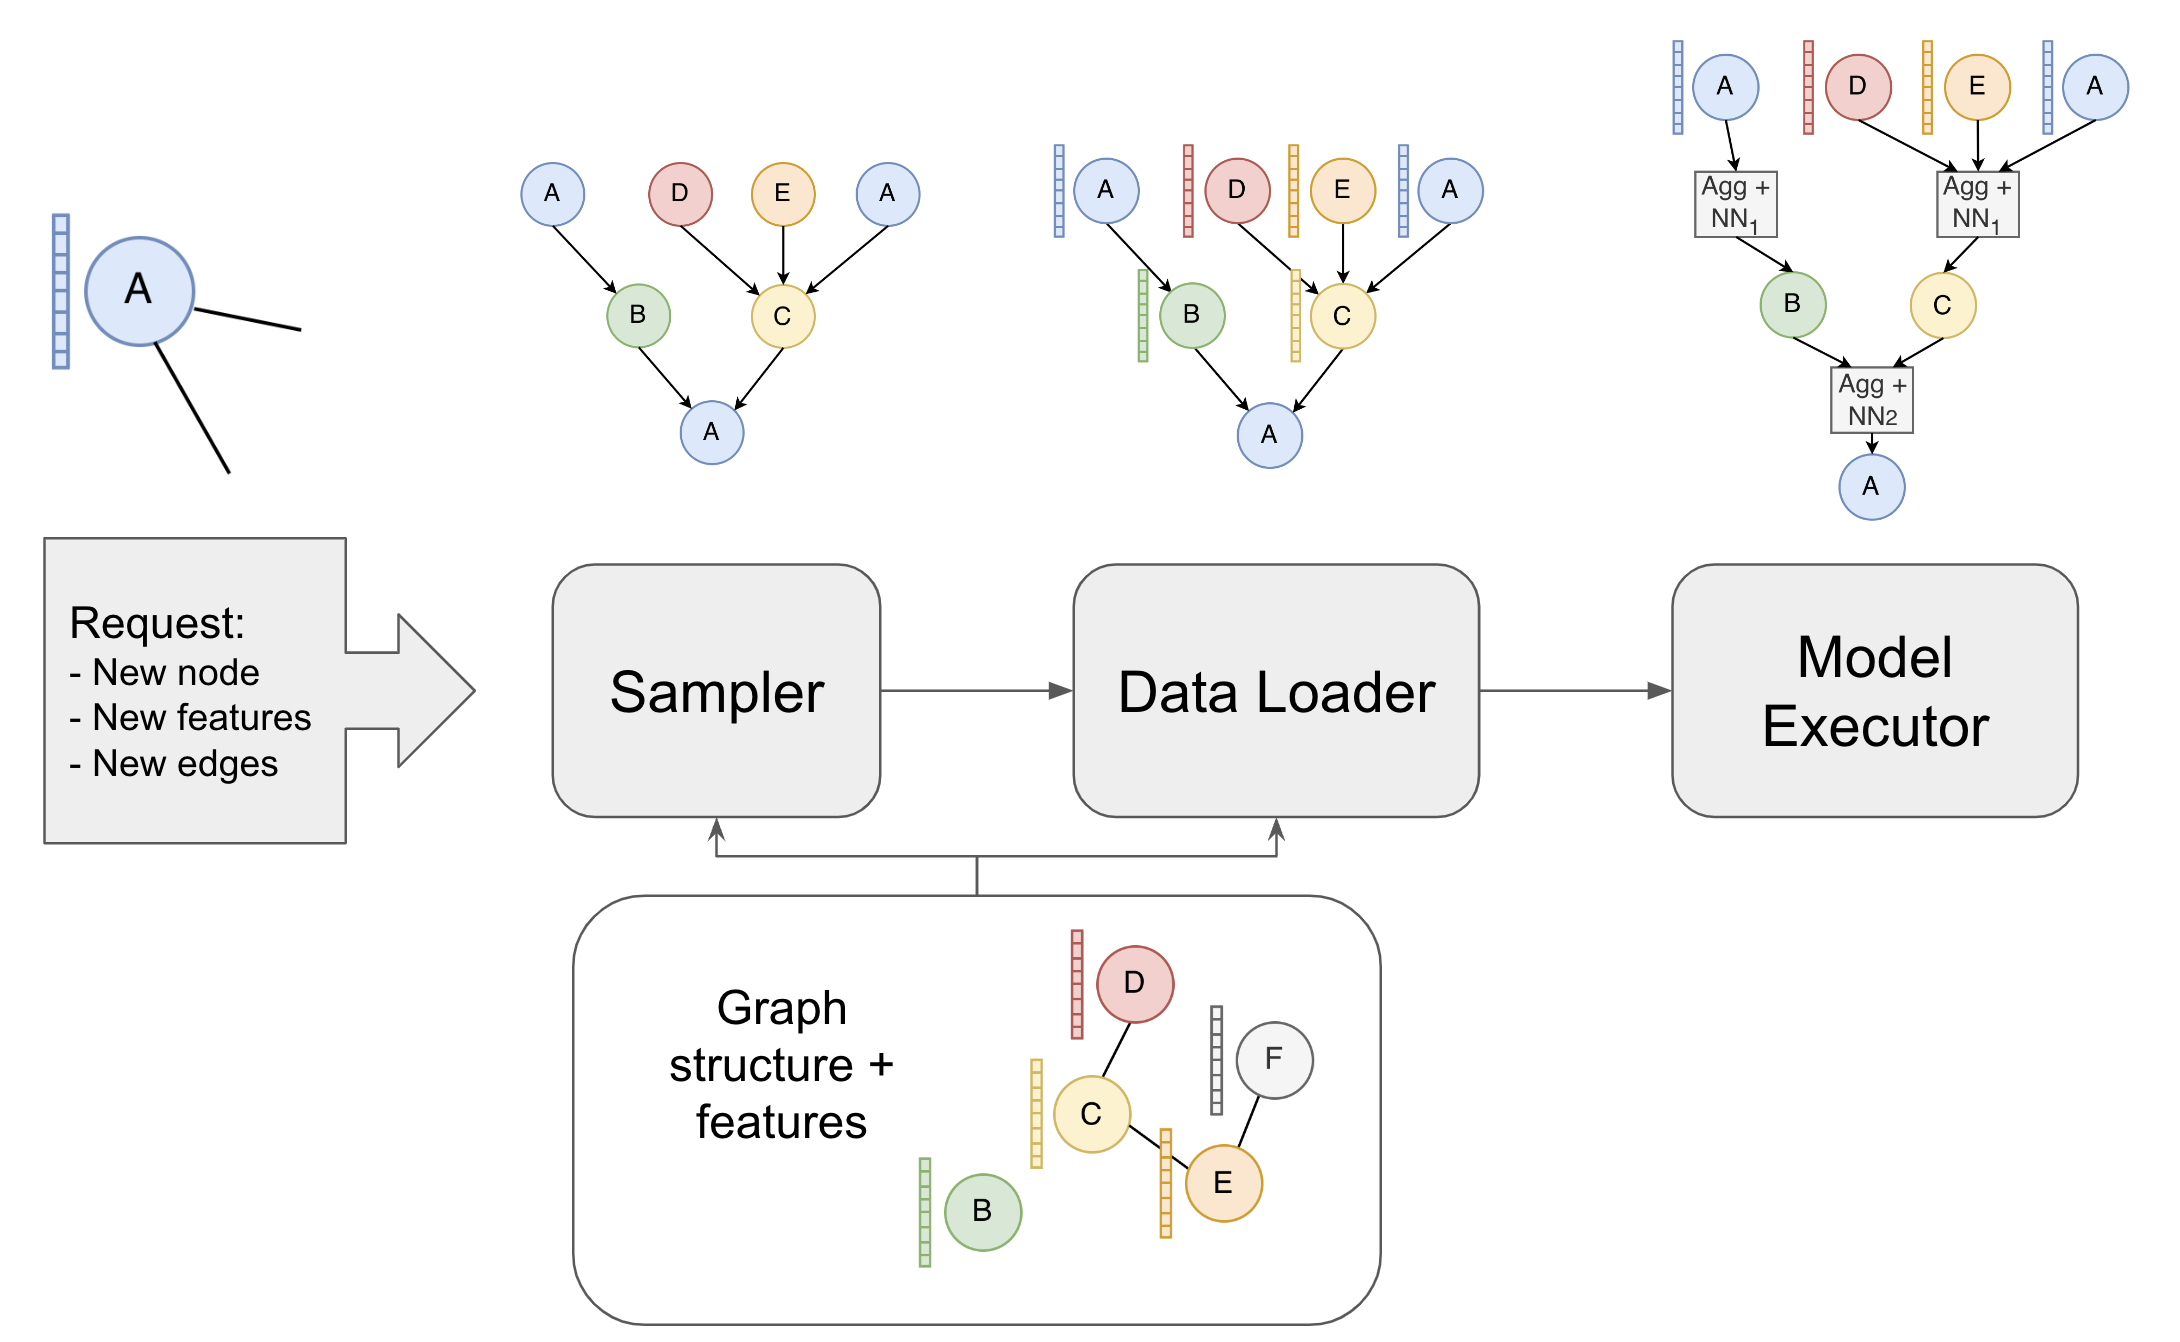
\includegraphics[width=\textwidth]{figures/Compute example.png}
    
    \caption{Online GNN Inference}
    \label{Compute Visualization}
\end{figure}    


%%%%%%%%%%%%%%%%%%%%%%%%%%%%%%%%%%%%%%%%%%%%%%%%%%%%%%%%%%%%%%%%%%%%%%%%
\section{Inference vs. Training} \label{Background: Relation to training}
%%%%%%%%%%%%%%%%%%%%%%%%%%%%%%%%%%%%%%%%%%%%%%%%%%%%%%%%%%%%%%%%%%%%%%%%
In this section we analyze similarities and differences between the inference and training tasks and examine the effectiveness of relevant GNN training optimizations at inference time.

Mini-batch training is a popular technique for GNN training on large graphs where embeddings are only computed for a random subset of the graph per epoch \cite{BGL_2023}. 
This is as opposed to full graph training, where node embeddings and gradients are computed for the entire graph at once, similar to full graph inference.
Mini-batch training is analogous to online inference, and, aside from the high-level goal, the difference is that no backpropagation is needed for inference. We briefly look at prior optimizations for the sampling and data loading stages, with particular emphasis on the latter.

\subsubsection{Sampling Optimizations}
The \textit{neighborhood explosion} problem is a well-known issue in the sampling stage.
Since the size of $k$-hop neighborhoods is inherently exponential, constructing these neighborhood and corresponding computation graphs can be expensive. \textit{Neighborhood sampling} helps alleviate this problem by randomly selecting a fixed number or percentage of node neighbors during the sampling stage \cite{GraphSAGE_2017}. 
However, since this can produce a drop in model accuracy, works such as NextDoor \cite{NextDoor_2021} have proposed performing sampling on GPU rather than CPU, yielding significant speedups.
In our system we will leverage this GPU sampling approach.

\subsubsection{Data Loading Optimizations}

Prior GNN training works have observed that data loading can also be a significant bottleneck.
Bus bandwidth between host memory and GPUs can easily be saturated by GNN data loading. 
For reference, PCIe 3.0 16x and PCIe 4.0 16x unidirectional bandwidth is 16 GB/s and 32 GB/s respectively.
Meanwhile, given exponential neighborhood sizes and large feature dimensions, it is easy for transfers of several hundred megabytes to be required for each minibatch.
Therefore, gathering these features in CPU memory and copying them to the GPU can bottleneck training pipelines.

Since GNN models have relatively few parameters compared to traditional DNNs, GPU compute and memory can actually be underutilized during training. Thus several works have proposed caching node features in GPU memory so they no longer need to be copied over from host memory. We are particularly interested in the following GNN training systems implementing feature caches since we find that data loading is a several bottleneck during inference.

\begin{description}
    \item[PaGraph \cite{PaGraph_2020}] introduces \textit{static feature caching}, proposing a policy where the features of the highest degree nodes in the graph are stored on the GPU prior to training. This cache is \textit{static} since these features remain permanently in GPU memory until training concludes. A static cache can be used for inference and is low overhead, but has worse cache hit rates than dynamic caches.
    \item[GNNLab \cite{GNNLab_2022}] extends static caching to include a pre-sampling phase, where warmup epochs are run to determine what nodes are most often used and thus should be stored in the cache. Although the pre-sampling approach cannot be directly applied to inference, we build upon the idea of using frequency as a feature for determining cache residents in Section \ref{Design: Policy}.
    \item[BGL \cite{BGL_2023}] uses a dynamic FIFO cache and iterates over the graph in a roughly-BFS manner to exploit the FIFO cache. BGL's approach is reliant on controlling the node order during training time and thus cannot be applied to inference. However, BGL does introduce using NVLinks between GPUs to share cache resources, which we improve upon by enabling greater concurrency in Sections \ref{Design: Multi-GPU} and \ref{Design: Lock-free}.
\end{description}

\subsection{GNN Inference Challenges}
We observe that after adopting the GPU sampling and static caching techniques from GNN training systems, inference latency is still dominated by data loading operations. Figure \ref{GPU Sampling Latency Breakdown} illustrates these results. 

\begin{figure}[h!]
    \centering
    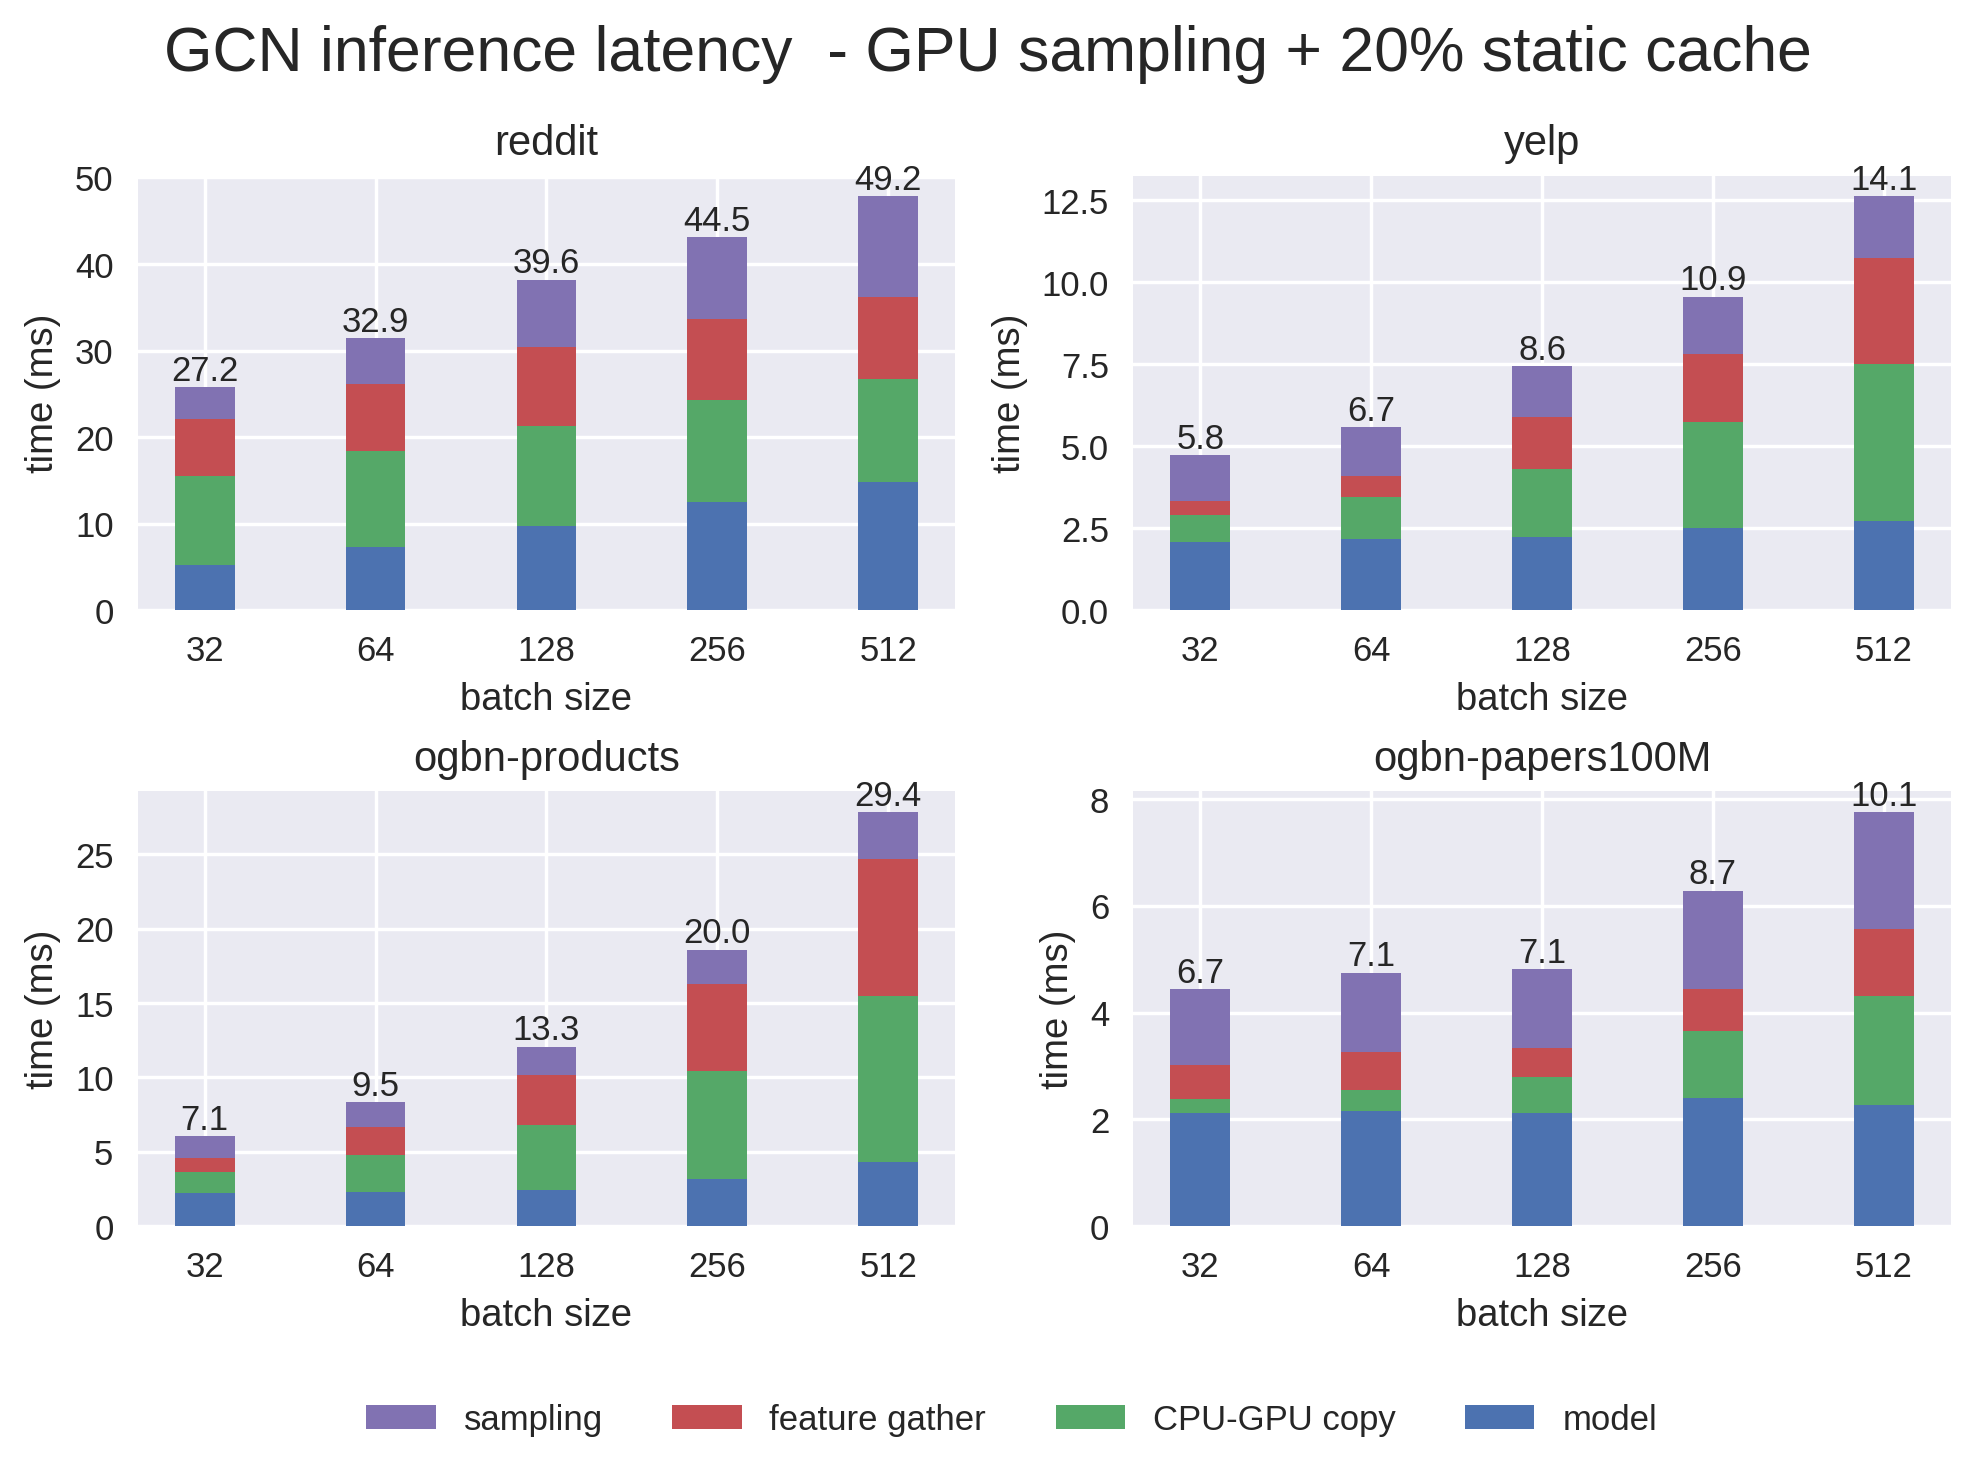
\includegraphics[width=0.8\textwidth]{figures/GCN_latency_breakdown_gpu_sampled_with_cache.png}
    
    \caption{Inference latencies for different graph datasets and request batch sizes (number of target nodes in request). Requests are served by a system using GPU sampling and a static cache large enough to hold 20\% of each graph dataset's node features. The test platform is detailed in Section \ref{Eval: Test hardware}}
    \label{GPU Sampling Latency Breakdown}
\end{figure}    

We identify key challenges with GNN inference, making it critical to carefully apply data loading optimizations. In particular,

\begin{enumerate}
    \item \textbf{Latency is a key metric at inference time}. During GNN training, throughput is far more important than latency. For example, many training systems try to hide data loading overheads by pipelining additional compute during data transfers. However, pipelining cannot hide latency. As a result, an efficient inference system must directly reduce data loading overhead.
    \item \textbf{Data loading is the key inference bottleneck}. As Figure \ref{GPU Sampling Latency Breakdown} shows, the data loading step is the bottleneck in terms of inference latency. This is actually mostly inference-specific, since at inference time there is no need to perform backpropagation, meaning that sampling and data loading comprise a larger percentage of inference latency. Furthermore, modern deep learning frameworks such as PyTorch \cite{PyTorch_2019} and TensorFlow \cite{tensorflow2015-whitepaper} offer optimizations that can be enabled at inference time, such as not tracking gradients, which skews this proportion further.
\end{enumerate}

As a result, we believe it is important to reduce data loading overheads by improving GPU feature caches.


% Reasons why we optimize data lodaing stage
% \begin{enumerate}
%     \item \textbf{Data loading comprises significant portion inference latency}
%     \item \item \textbf{Data loading latency cannot be hidden with pipelining}
%     \item \textbf{Data loading overhead scales with feature dimension}
% \end{enumerate}



  % %%%%%%%%%%%%%%%%%%%%%%%%%%%%%%%%%%%%%%%%%%%%%%%%%%%%%%%%%%%%%%%%%%%%%%%%
\chapter{Motivation}
%%%%%%%%%%%%%%%%%%%%%%%%%%%%%%%%%%%%%%%%%%%%%%%%%%%%%%%%%%%%%%%%%%%%%%%%

%%%%%%%%%%%%%%%%%%%%%%%%%%%%%%%%%%%%%%%%%%%%%%%%%%%%%%%%%%%%%%%%%%%%%%%%
\section{GNN Inference Challenges and Opportunities}
%%%%%%%%%%%%%%%%%%%%%%%%%%%%%%%%%%%%%%%%%%%%%%%%%%%%%%%%%%%%%%%%%%%%%%%%
Although GNN inference has similarity to training, inference has unique challenges and opportunities not present in the training setting. 
In this section we examine these differences in detail, discuss inference bottlenecks based on concrete experiments, and motivate our approach based on an analysis of naive solutions.

\subsection{Inference-specific Challenges}
Leveraging approaches from existing training systems present several key challenges, namely:

\begin{enumerate}
    \item \textbf{Latency is a key metric at inference time}. This is not the case during training. During training, throughput is a far more important metric than latency. For example, many training systems avoid data loading bottlenecks using pipelining. However, pipelining cannot hide latency.
    \item \textbf{Node ordering cannot be controlled}. While training systems can use 
    \item \textbf{No backpropagation leads to sampling and data loading dominating inference latency}. 
\end{enumerate}

\begin{figure}[h!]
    \centering
    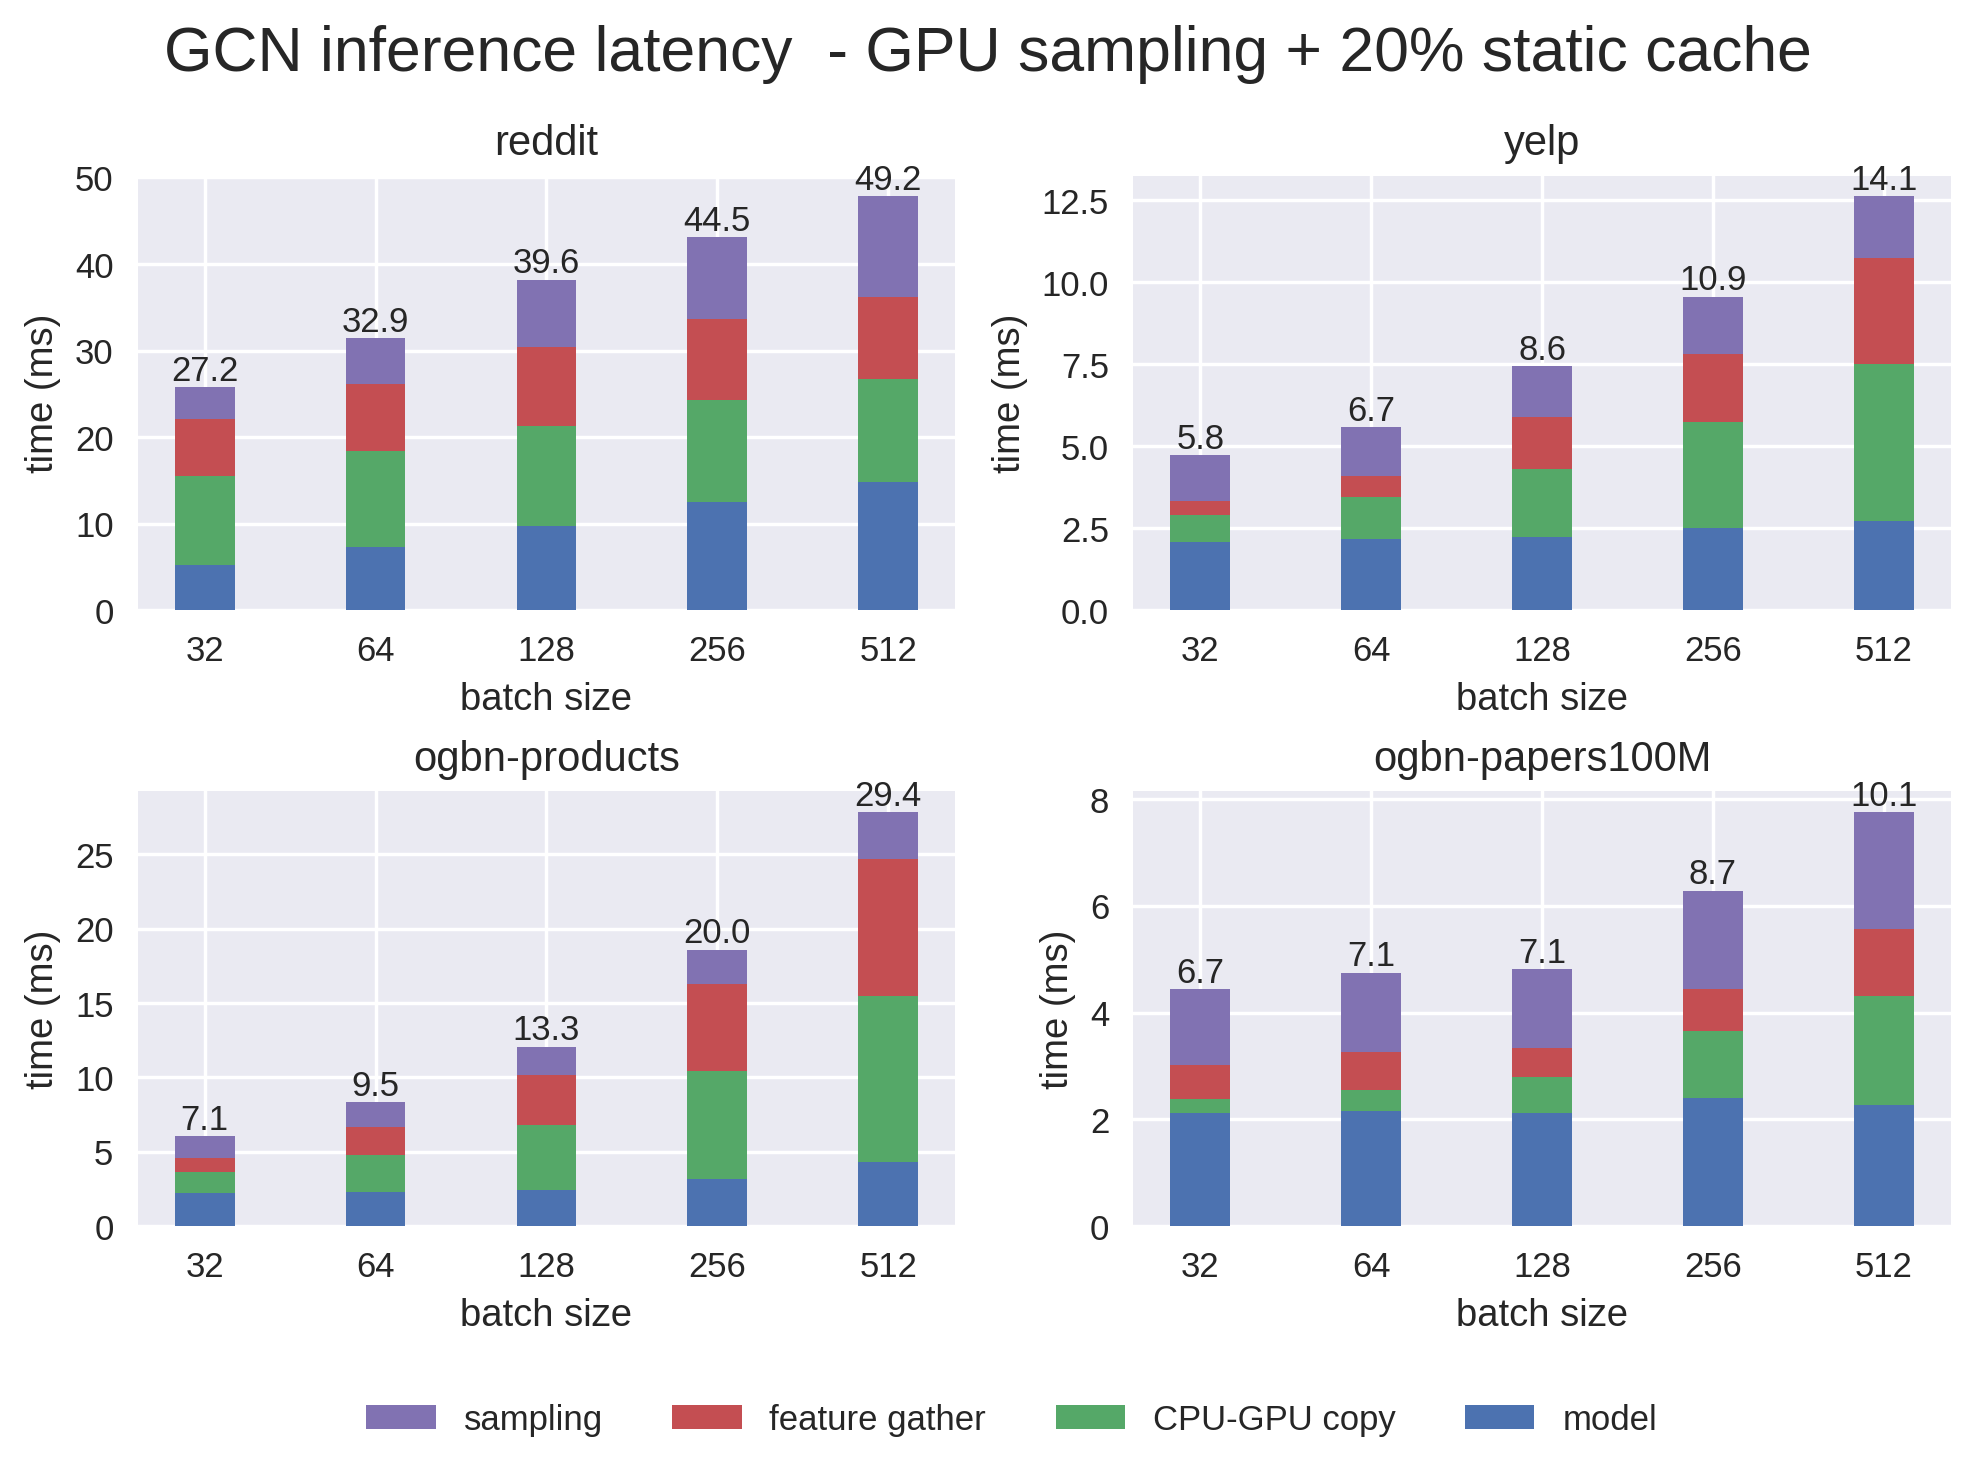
\includegraphics[width=\textwidth]{figures/GCN_latency_breakdown_gpu_sampled_with_cache.png}
    
    \caption{Inference latencies for different graph datasets and request batch sizes (number of target nodes in request). Requests are served by a system using GPU sampling and a static cache large enough to hold 20\% of the graph's node features.}
    \label{GPU Sampling Latency Breakdown}
\end{figure}    

\begin{enumerate}
    \item Inference latency is important, here is example
    \item Existing solutions don't work for inference \& 
         Data loading is the bottleneck after using GPU sampling
    \item Subgraph locality opportunity means we can exploit dynamic cache
    \item Challenging because need to meet latency and throughput SLAs
    \item Go into our solution
\end{enumerate}

% %%%%%%%%%%%%%%%%%%%%%%%%%%%%%%%%%%%%%%%%%%%%%%%%%%%%%%%%%%%%%%%%%%%%%%%%
% \section{Towards Dynamic Caching}
% %%%%%%%%%%%%%%%%%%%%%%%%%%%%%%%%%%%%%%%%%%%%%%%%%%%%%%%%%%%%%%%%%%%%%%%%


\subsection{Subgraph Locality of Inference Requests}
% Discuss when and why inference requests may have locality
Our key observation is that inference requests can 

\subsection{Naive Approaches to Dynamic Caching}
% Explain why LFU/LRU doesn't work, same with the prefetch based approach


% \begin{figure}[h!]
%     \centering
%     % \includegraphics[width=\textwidth]{stamp_graphs.png}
    
%     \caption{[todo add graphs showing latency breakdown for different graphs ]}
%     \label{Baseline Latency Breakdown}
% \end{figure}    

% \begin{figure}[h!]
%     \centering
%     % \includegraphics[width=\textwidth]{stamp_graphs.png}
    
%     \caption{[todo add graphs showing latency breakdown for different graphs ]}
%     \label{Static Cache Latency Breakdown}
% \end{figure}    




\subsection{Online Inference Challenges}
\begin{enumerate}
    \item Can't pipeline latency
    \item No backprop makes data loading larger percentage
    \item Opportunity because of subgraph requests, cite QGraph and stuff
\end{enumerate}

\subsection{Limitations}
[TODO move this elsewhere]
Our system currently does not combine new inference requests into the existing graph or retrain the GNN to accommodate for new requests. 
Instead, we look only at GNN computation and investigate how to efficiently compute new embeddings. 
Integrating new nodes into the existing graph and dealing with challenges such as consistency are both orthogonal and out of scope of this work, but would be an interesting and natural extension.

%%%%%%%%%%%%%%%%%%%%%%%%%%%%%%%%%%%%%%%%%%%%%%%%%%%%%%%%%%%%%%%%%%%%%%%%
\section{GNN Inference Challenges}
%%%%%%%%%%%%%%%%%%%%%%%%%%%%%%%%%%%%%%%%%%%%%%%%%%%%%%%%%%%%%%%%%%%%%%%%

  %%%%%%%%%%%%%%%%%%%%%%%%%%%%%%%%%%%%%%%%%%%%%%%%%%%%%%%%%%%%%%%%%%%%%%%%
\chapter{Design}
%%%%%%%%%%%%%%%%%%%%%%%%%%%%%%%%%%%%%%%%%%%%%%%%%%%%%%%%%%%%%%%%%%%%%%%%
Our system leverages a novel approach to dynamic cache updates to serve GNN inference requests with low-latency. 
We target single-machine, multi-GPU inference systems and build upon caching techniques in GNN training systems discussed in the previous chapter. 
In this chapter, we address three key research questions:
\\ \\
\noindent \textbf{RQ1: How can GPU feature caches effectively capture GNN inference patterns?} \\
Section \ref{Design: Towards Dynamic Caching} describes opportunities for dynamic caches to outperform existing static caches at inference time and highlights shortcomings of naive approaches. Section \ref{Design: Policy} proposes a frequency-based cache admission and eviction policy that produces better cache hit rates that static baselines while offering a path towards efficient update operations.
\\ \\
\noindent \textbf{RQ2: How can the impact of dynamic cache updates on request-response latency be minimized?} \\
Section \ref{Design: Async Update} details how we derive an asynchronous cache update mechanism based on profiling of a naive cache update mechanism using "prefetching". By carefully engineering this asynchronous cache update, we are able to hide cache update operations that would otherwise negatively impact tail latency.
\\ \\
\noindent \textbf{RQ3: How can we effectively leverage concurrency (multithreading, multi-GPU) to produce scalable inference?} \\
Since asynchronous updates synchronized using naive locking can produce blocking behaviors when pipelined (and thus no longer be truly asynchronous), we propose a lock-free mechanism to perform cache updates, discussed in Section \ref{Design: Lock-free}.
Lastly, Section \ref{Design: Multi-GPU} describes how we extend our system to support multiple GPUs connected by NVLinks and share a single logical cache.

% Our system implements the same frequency-based admission and eviction policy from the prefetching baseline but combines it with an asynchronous cache update mechanism to reduce tail latencies. 
% Section \ref{Design: Policy} analyzes this policy in more detail and Section \ref{Design: Async Update} describes how asynchronous updates take place. 
% Since asynchronous updates synchronized using naive locking can produce blocking behaviors when pipelined (and thus no longer be truly asynchronous), we propose a lock-free mechanism to perform cache updates, discussed in Section \ref{Design: Lock-free}.
% Lastly, Section \ref{Design: Multi-GPU} describes how we extend our system to support multiple GPUs connected by NVLinks and share a single logical cache.


%%%%%%%%%%%%%%%%%%%%%%%%%%%%%%%%%%%%%%%%%%%%%%%%%%%%%%%%%%%%%%%%%%%%%%%%
\section{Towards Dynamic Caching} \label{Design: Towards Dynamic Caching}
%%%%%%%%%%%%%%%%%%%%%%%%%%%%%%%%%%%%%%%%%%%%%%%%%%%%%%%%%%%%%%%%%%%%%%%%
One of our key observations is that effective caching is pivotal to reducing data loading costs, and dynamic cache policies can enable better cache hit rates.
We define a \textit{dynamic} cache policy as one that swaps node features in and out of GPU memory over time. We identify two key opportunities  that dynamic caches can capture that static caches neglect:
\begin{description}
    \item[Inference request locality] Inference requests generate large neighborhoods during the $k$-hop neighborhood generation process. Due to this, if inference requests being "close" in the graph have reasonable semantic meaning in the real world, then we can expect inference requests to exhibit locality. For example, in a social network graph there may be clusters of users who are in a similar geographic area. These users may have more activity and generate more inference requests during the daytime, meaning that subgraphs become "hot" at different points in time. Prior work in the graph processing space has also noted the importance of request locality in domains such as traffic prediction or knowledge graph mining \cite{QGraph_2018}.
    % For example [traffic], [over time], [popular products]
    \item[Sampling patterns] Since GNNs require $k$-hop neighborhoods, a policy that caches node features based solely on node out-degree can neglect nodes that are actually likely to be used. For example, a low-degree node that is directly adjacent to several high-degree nodes is likely to be similarly "hot" to its high-degree neighbors. Additionally, certain GNN architectures leverage specific parameters when building neighborhoods, such as by assigning edge weights [cite edge weight].
\end{description}

\subsection{Why Traditional Dynamic Caches are Ineffective}
An intuitive first step towards dynamic caches is to consider using traditional cache eviction policies such as LRU, LFU, or FIFO. However, many of these approaches have too much overhead to be effective for GNN inference. 

In the GNN inference case, each request (comprising anywhere from one to several hundred target nodes) can generate $k$-hop neighborhoods of hundreds of thousands of nodes.
As a result, the overhead of cache replacement heuristics can quickly overtake any performance gains from improved cache hit rates. For example, the traditional implementation of an LRU cache using a linked list and hash table to track elements will severely bottleneck GNN inference. Consider the following back of the envelope calculation. We find that a naive GNN inference system can generally serve requests with $< 100$ ms latency. Assuming a cache put or get takes only $500$ ns, as is the case with many publicly available LRU cache implementations [todo cite https://github.com/hashicorp/golang-lru], for one request this requires $~100,000 \text{ nodes} * ~500 \text{ ns} = 50 \text{ ms}$. Given that this would add at least $50\%$ to our original inference latency, such overhead is clearly unacceptable. 

To handle potentially huge neighborhood sizes, a key requirement for a cache policy is to be easily parallelizable. A frequency-based heuristic meets this criteria and has been shown to be effective in the GNN setting a training time, with GNNLab's pre-sampling approach \cite{GNNLab_2022}. Even so, the traditional LFU policy can still struggle versus a static cache baseline as it requires some kind of sorting or top-$k$ operation for each request served.

Furthermore, large neighborhood sizes require us to also consider a cache admission policy. If only a cache eviction policy is used, it is easy for a "one-hit wonder" to be brought in among hundreds of thousands of other nodes and waste cache space.

Note that static caches do not suffer from these performance problems since checking for cache hits is easily implemented using tensor operations.
% However, since LFU is only an eviction policy 
% only eviction policies, in practice can be subject to one-hit wonders
% Prefetch based approach

% We draw a distinction between cache policy and cache mechanism.

%%%%%%%%%%%%%%%%%%%%%%%%%%%%%%%%%%%%%%%%%%%%%%%%%%%%%%%%%%%%%%%%%%%%%%%%
\section{Frequency-based Admission \& Eviction Policy} \label{Design: Policy}
%%%%%%%%%%%%%%%%%%%%%%%%%%%%%%%%%%%%%%%%%%%%%%%%%%%%%%%%%%%%%%%%%%%%%%%%
Motivated by our observations in the previous section, in this section we propose a simple frequency-based cache admission and eviction policy. Then, we briefly illustrate the improved cache hit rates of this policy when using a naive, strawman cache update mechanism.

The goal of our policy is straightforward: to admit the most frequently occurring node features and evict the least frequent node features within a particular time window. Implementing this heuristic requires tracking node frequencies and decaying them over time.

In our implementation node frequencies are tracked in a buffer in GPU memory. By tracking frequencies on the GPU rather than the host, our system avoids an additional device to host copy, since computation graphs are built on GPU. The frequency buffer has length equal to the number of nodes in the graph.
Each index in the buffer corresponds to a node, and the value is a counter that gets incremented whenever the node's feature is required.
To reduce GPU memory usage, this buffer uses only one byte for each node. 
However, the size of the buffer still scales with the number of nodes in the graph. We note that frequencies can also be tracked using a probabilistic data structure like a counting bloom filter \cite{Bloom_Filter_2000} or count-min sketch \cite{CountMinSketch_2005}, but we do not implement this.
Using such a probabilistic data structure actually makes it easier to add new nodes into the graph, since there is no buffer that needs to be resized.
We leave this as future work.

To capture changes in node frequencies, the count buffer must decay over time.
This is implemented by periodically dividing all counts in the buffer by two, a technique adapted from TinyLFU \cite{TinyLFU_2014} which produces exponential decay.
A nice property of exponential decay is that it is easy to bound the maximum possible count and fit it within the one byte constraint. 
Additionally, the decay can be implemented as a bit shift for better performance and still works with a count-min sketch or counting bloom filter.

% There are many policy choices regarding how exactly to choose which nodes to evict or admit. 
% For example, a policy could weight both a node's degree as well as its recent frequency when making admission decisions. 
% The weighting of node degree versus frequency is a user-adjustable knob in our system, but for the evaluation in Chapter \ref{Evaluation}, we use only frequency when evaluating frequency-based approaches.


\subsection{Strawman Prefetching Mechanism}
Given the above policy, an actual implementation must choose some mechanism by which to perform cache updates and perform the top-$k$ frequency calculations. For example, LFU is traditionally implemented by tracking most common elements using a heap and evicting/admitting into the cache per-request; however, as we saw earlier this can harm inference latency. We present an alternative strawman mechanism essentially replaces the static cache with a new one every $k$ requests according to the above policy. We call this alternative baseline mechanism our \textit{prefetching} strawman. 

In particular, every $k$ requests the cache is entirely replaced with the most common nodes that appeared in the previous $k$ requests. This means that node features are pulled to the GPU feature cache and request handling must be paused as necessary. 

The key idea is that this strawman maintains the low overhead nature of a static cache while improving cache hit rates, but every $k$ requests it incurs a large penalty due to a cache update. This cache update penalty produces significant tail latency, which we analyze in the next section.

%%%%%%%%%%%%%%%%%%%%%%%%%%%%%%%%%%%%%%%%%%%%%%%%%%%%%%%%%%%%%%%%%%%%%%%%
\section{Asynchronous Cache Update mechanism} \label{Design: Async Update}
%%%%%%%%%%%%%%%%%%%%%%%%%%%%%%%%%%%%%%%%%%%%%%%%%%%%%%%%%%%%%%%%%%%%%%%%
 
To eliminate tail latencies associated with the prefetching strawman, our system uses an asynchronous cache update mechanism, moving cache update operations off the critical path when responding to inference requests.
Table \ref{Update latencies} provides a breakdown of average cache update overheads for a selected dataset, ogbn-products, during a single-threaded inference execution. The prefetching-based update produces significant tail latency, in this case increasing response latency by more than a third when the update occurs.

\begin{table}[h!]
    \begin{center}
        \textbf{Breakdown of Average Cache Update Overhead}
        \begin{tabular}{|c c c|} 
        \hline
        \textbf{Operation} & \textbf{Time (ms)} & \textbf{Percent of Update Time} \\ [0.5ex] 
        \hline\hline
        Update cache metadata & 2.7 & 47\%  \\
        \hline
        Feature copy & 2.2 & 38\% \\
        \hline
        Compute most common features & 0.6 & 10\% \\
        \hline
        Misc. (locking, device sync, etc.) & 0.2 & 3.5\% \\
        \hline
        Total & 5.7 & \\
        \hline
        \end{tabular} \\
        Average inference latency without update: 12.7 ms
    \end{center}
    
    % ogbn-products, uniform sampling, batch size 256, total latency 
    \caption{Breakdown of time spent on operations when performing cache update.
    These are the operations that contribute to significant tail latency with the prefetching policy.
    }
    \label{Update latencies}
\end{table}

The largest contributors to cache update overhead in the prefetching strawman are copying new features from host memory to GPU memory and updating cache metadata.
Using this profiling information, we motivate three design decisions.
\textbf{(1)} Rather than prefetching features to move into GPU memory, we move features into the cache only when they are needed by inference requests, similar to traditional cache eviction policies. 
\textbf{(2)} To sidestep overheads due to updating cache metadata, we move metadata updates to a separate host thread and CUDA stream (synchronization is discussed in Section \ref{Design: Lock-free}).
\textbf{(3)} Lastly, we can compute the most common features (in practice a top-$k$ operation) in a separate CUDA stream.

% \begin{enumerate}
%     \item Compute set of cache candidates
%     \item Python process places torch tensor into queue, picked up by C++ thread
%     \item Removed from queue when model execution finishes to avoid ballooning memory usage
%     \item Also experimented with updating counts/doing other operations in C++ thread
% \end{enumerate}

\subsection{Computing Cache Candidates}
To support moving features into the cache only when they are needed by inference requests while adhering to the desired policy, we introduce the idea of \textit{cache candidates}, a set of node ids computed every $k$ requests. When a cache miss occurs and new node features are copied to the GPU from host memory, the new features are checked against the set of cache candidates. If a feature corresponds to a node that is a cache candidate, then it will replace a non-cache candidate present in the cache. This is possible since at any given point in time, the number of cache candidates is equal to the size of the cache.



\subsection{Performing Cache Updates}
The actual cache update itself is handled by a separate host thread and CUDA stream than the one handling inference requests. 

One important aspect of this approach is that the cache update should occur during the model forward pass.
The key insight is that node features are already present in GPU memory for the model forward pass and thus are assumed to fit in GPU memory fine.
However, if the asynchronous update thread holds on to these tensors longer than the model forward pass would normally take, memory usage can be inflated. 
We avoid this problem by allowing the model forward pass to have full ownership of any node features required for computation.
If the model forward pass for a given inference request is completed and the cache update has not started, then the cache update will be ignored.

To further avoid contention of GPU compute due to cache updates happening concurrently with model computation, we assign the cache update operations to a lower priority CUDA stream than model computation.

%%%%%%%%%%%%%%%%%%%%%%%%%%%%%%%%%%%%%%%%%%%%%%%%%%%%%%%%%%%%%%%%%%%%%%%%
\section{Lock-free Cache Updates} \label{Design: Lock-free}
%%%%%%%%%%%%%%%%%%%%%%%%%%%%%%%%%%%%%%%%%%%%%%%%%%%%%%%%%%%%%%%%%%%%%%%%
Asynchronous cache updates naturally raise concerns about correctness and performance due to concurrency. While naive locking may initially be adequate, at scale this may not be the case. In this section we look at a novel lock-free approach using \textit{masking} to avoid lock contention due to cache updates.


Consider the case where we would like our system to be pipelined to maximize throughput. Since the data loading stage requires reading from the cache, we must be careful about synchronization between cache updates and data loading since cache updates are not atomic.
\begin{figure}[h!]
    \centering
    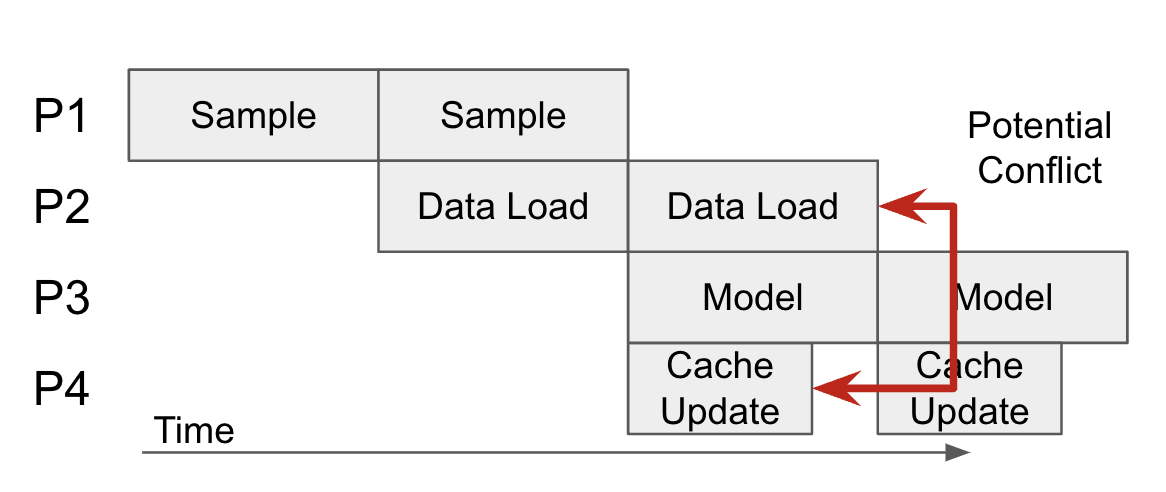
\includegraphics[width=0.85\textwidth]{figures/Pipeline no lock.png}
    \caption{[todo Lock conflict p99 latency]}
    \label{Impl: Conflict pipeline}
\end{figure}     
A case such as the one illustrated in Figure \ref{Impl: Conflict pipeline} can lead to cache readers reading the wrong feature from the cache if a cache update changes the cache buffer before the reader completes. 

A naive approach is to use mutual exclusion, such as with a reader-writer lock, but this can lead to asynchronous updates having equivalent performance to the original synchronous variety. Figure \ref{Impl: Contended pipeline} illustrates this effect. In this example, by enforcing mutual exclusion between the data loading thread and cache update thread, the second inference request is forced to wait on the cache update from the first inference request, meaning the latency of the first cache update was simply "passed along".

\begin{figure}[h!]
    \centering
    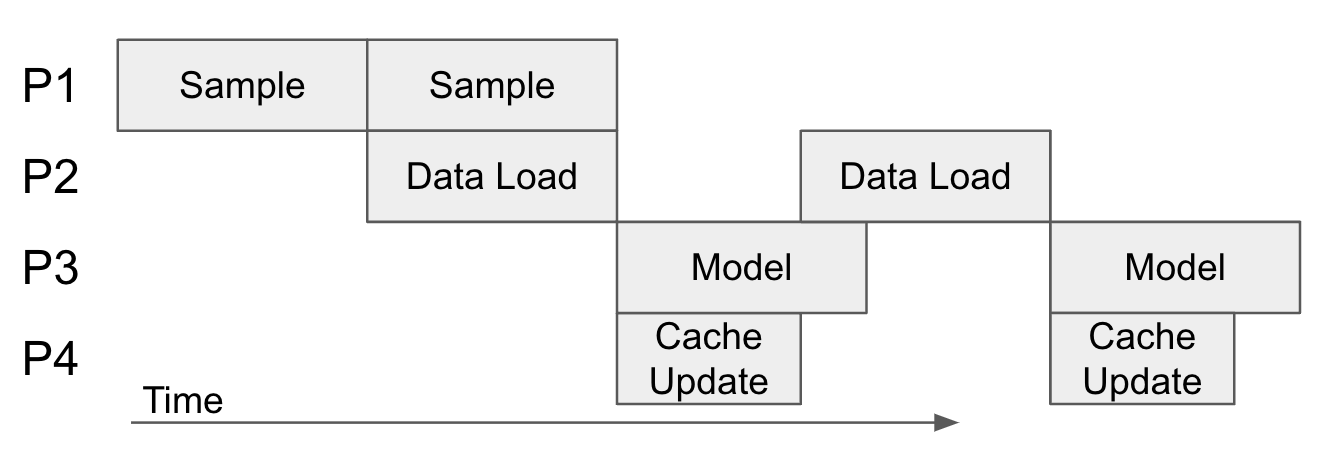
\includegraphics[width=\textwidth]{figures/Pipeline with lock.png}
    \caption{[todo Lock conflict p99 latency]}
    \label{Impl: Contended pipeline}
\end{figure}    

Even with a read-preferring or write-preferring reader-writer lock, eventually it must be the case that a cache read waits for a cache update, causing this "latency passing" behavior.  

\subsection{Masked Updates}
Motivated by the key observation that readers should be wait-free but writers can wait, we introduce a novel alternative to mutual exclusion in this situation. In our approach, which we call \textit{masking}, cache updates preemptively \textit{mask away} cache entries from cache readers and only perform updates once these cache entries will no longer be used by readers. 

Note that we assume only one thread performs a cache update at a time (per GPU), which is enforced by a simple mutex per GPU. If a cache update thread fails to acquire the lock, the update is thrown away.

To perform masked updates, we first add a \textit{mask} tensor to our cache metadata, which indicates for each node in the graph whether it is present in the cache (1 for present, 0 for not).

Then, for each logical thread of execution in the system, we initialize a start and finish atomic integer that just tracks whether the thread is currently performing a cache read.
When reading from the cache, threads will first increment their respective start atomic and then check the cache mask and only look in the cache for node ids where the mask indicates it is present.
Once the cache read is finished, the finish atomic is incremented.
Algorithm \ref{Design: Alg: Cache Read} summarizes this procedure.

When a cache update needs to occur, the writer will first blind write zeros into the cache mask for any node ids that will be evicted from the cache. 
Once the blind write has completed, the writer will then capture the value of all start atomics.
The writer capturing these values serves as a linearization point, as the writer will wait on the finish atomics until any in progress reads complete. 
At this point the cache writer is certain that any cache indices that will be replaced are no longer in use by any cache readers.
Algorithm \ref{Design: Alg: Cache Write} summarizes this procedure.


% declaration of the new block
\algblock{ParFor}{EndParFor}
% customising the new block
\algnewcommand\algorithmicparfor{\textbf{parallel for}}
\algnewcommand\algorithmicpardo{\textbf{do}}
\algnewcommand\algorithmicendparfor{\textbf{end\ parallel for}}
\algrenewtext{ParFor}[1]{\algorithmicparfor\ #1\ \algorithmicpardo}
\algrenewtext{EndParFor}{\algorithmicendparfor}

\begin{minipage}{0.4\textwidth}
    \begin{algorithm}[H]
        \centering
        \caption{Cache Read} \label{Design: Alg: Cache Read}
        \footnotesize
        \begin{algorithmic}[1]
        \Procedure{Read}{$node\_ids$}
            \State $i \gets \text{ Reader thread id}$
            \State $S[i] \gets S[i] + 1$
            \ParFor{$node\_id \in ids$}
                \If{$mask[node\_id] = 1$}
                    \State Do cache read for $node\_id$
                \EndIf
            \EndParFor
            \State $F[i] \gets F[i] + 1$
        \EndProcedure
        
        \end{algorithmic}
    \end{algorithm}
\end{minipage}
\hfill
\begin{minipage}{0.5\textwidth}
        \begin{algorithm}[H]
            \centering
            \caption{Cache Write} \label{Design: Alg: Cache Write}
            \footnotesize
            \begin{algorithmic}[1]
            \Procedure{Update}{$admit\_nids, evict\_nids$}
                \State $mask[evict\_nids] = 0$
                \For{$reader\_id \in reader\_ids$}
                    \State $s'[reader\_id] \gets s[reader\_id]$
                \EndFor
                \While{$\exists id \in reader\_ids : s'[id] < f[id]$}
                    \State Wait
                \EndWhile
                \State Do cache update
                \State $mask[admit\_nids] = 1$
            \EndProcedure
            
            \end{algorithmic}
        \end{algorithm}
\end{minipage}

\begin{figure}[h!]
    \centering
    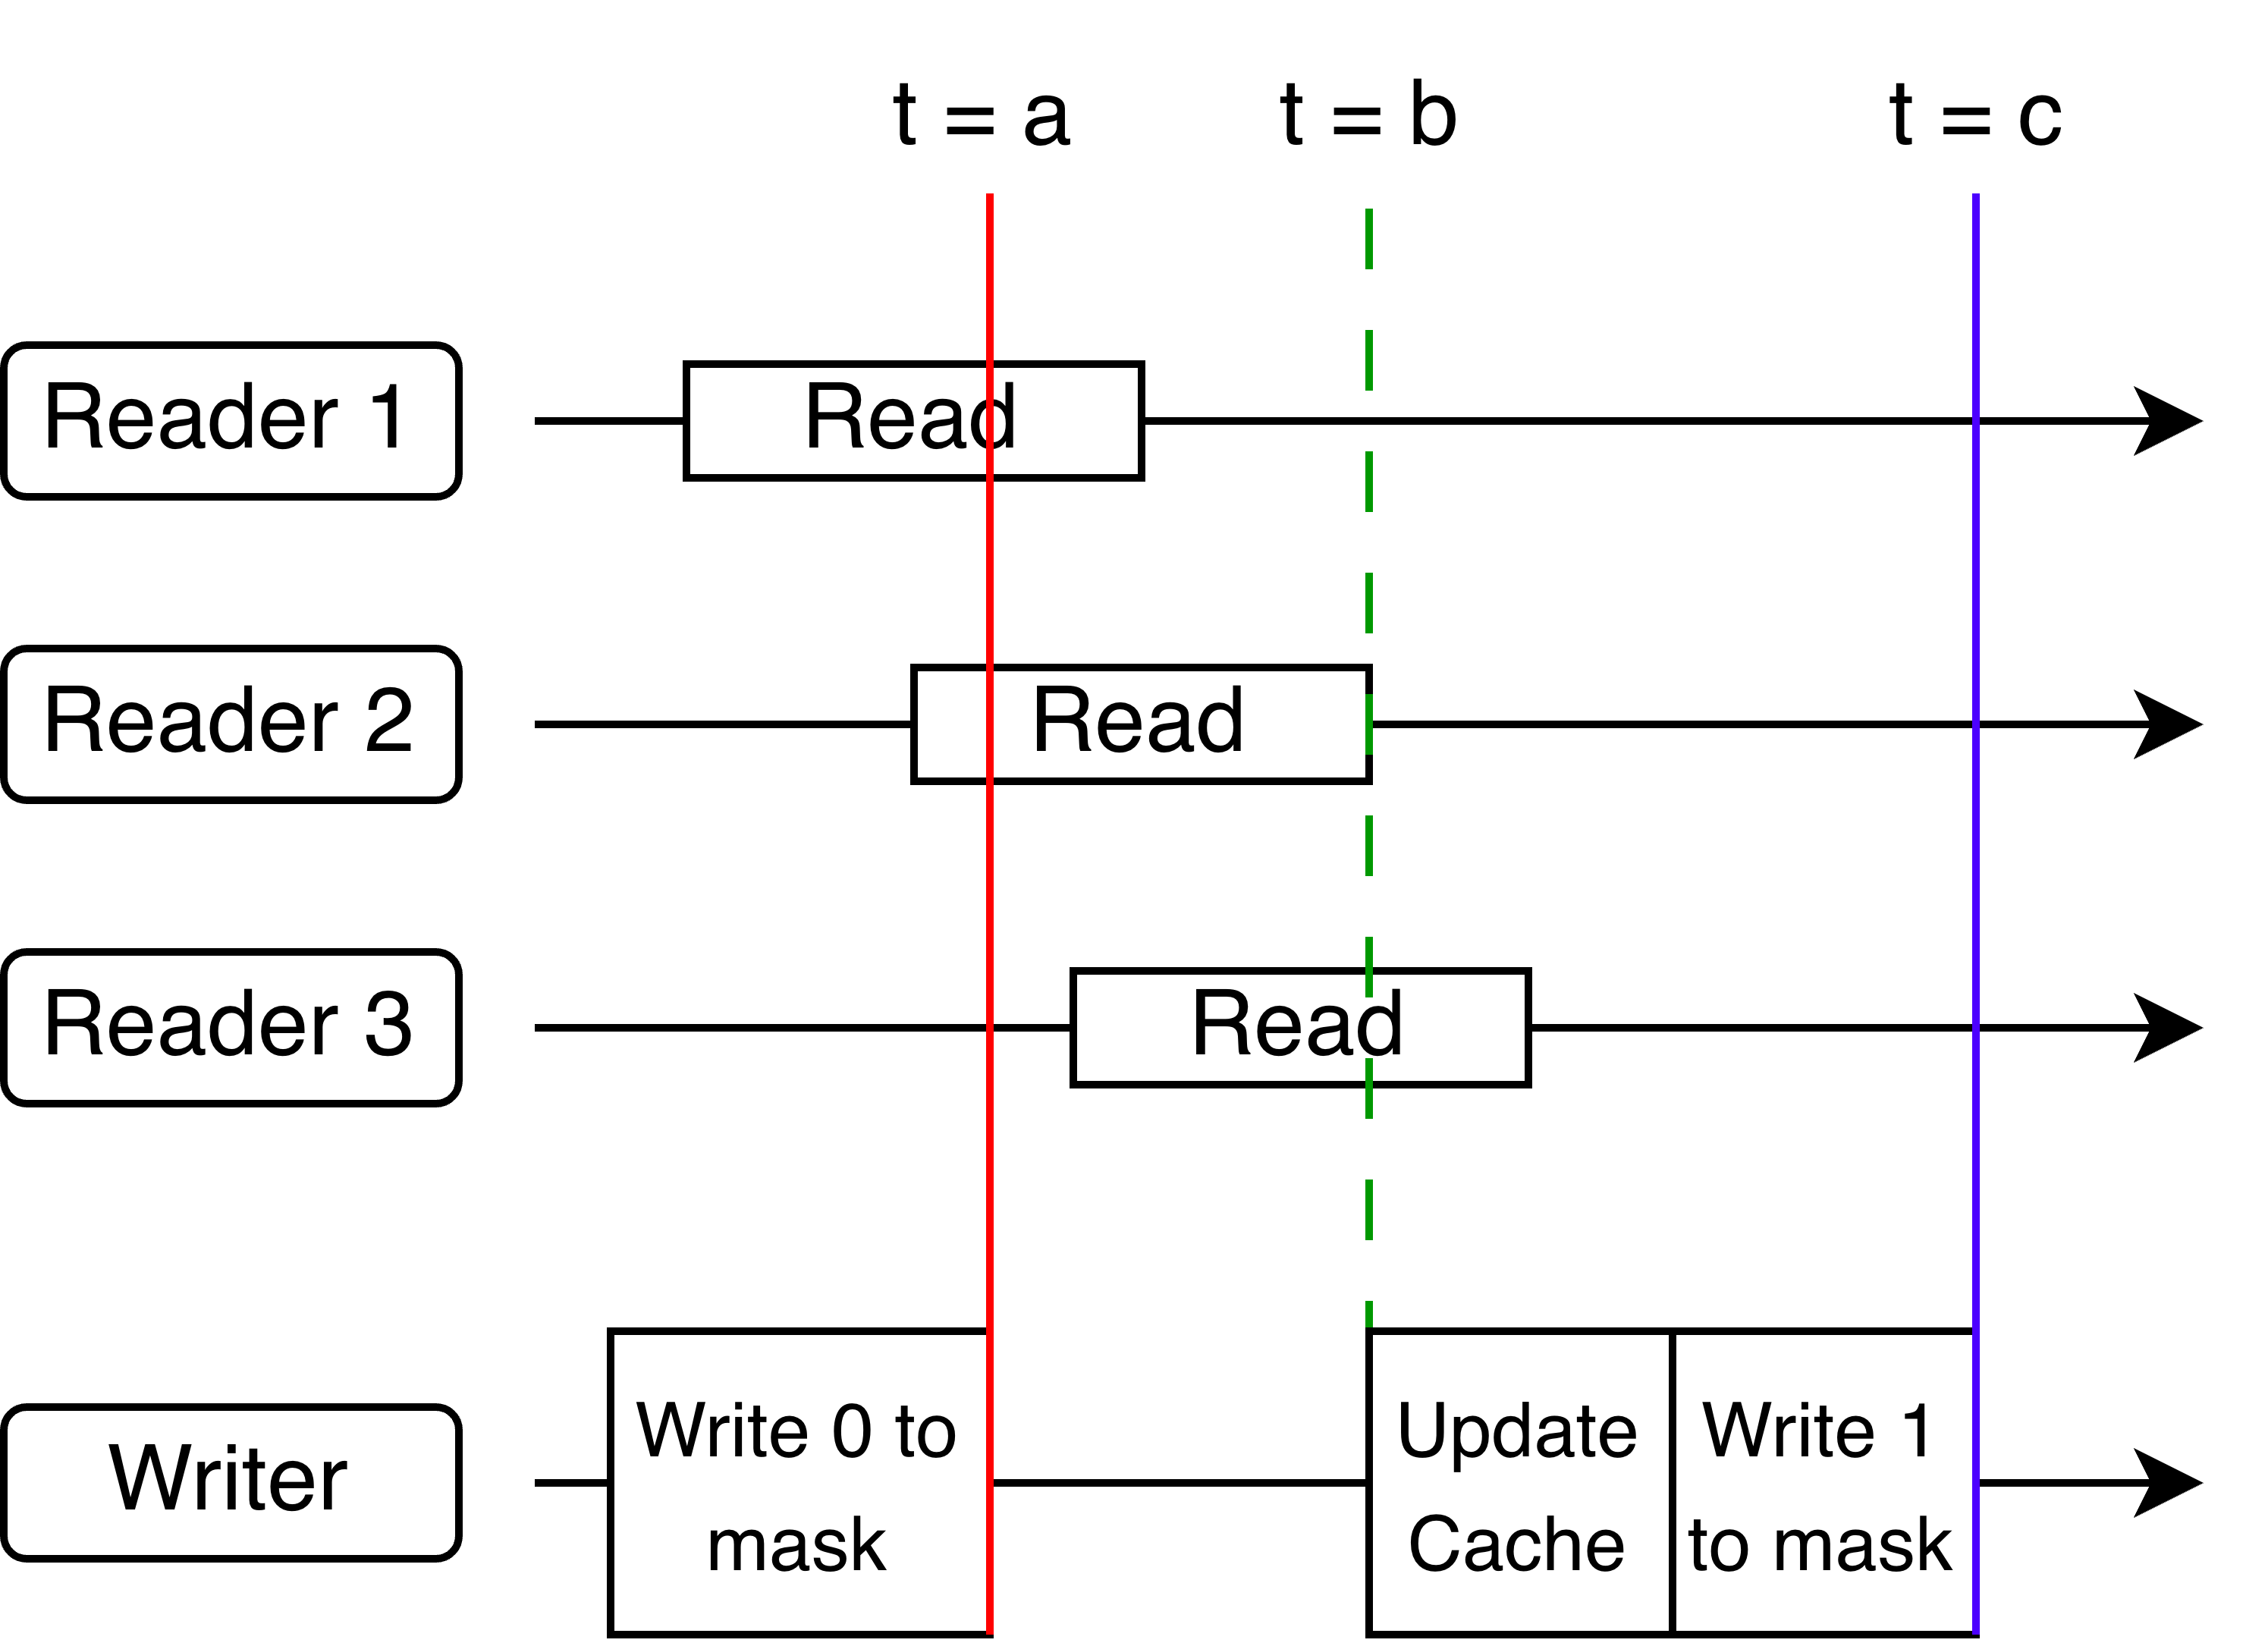
\includegraphics[width=0.7\textwidth]{diagrams/group_meeting_gnn-Multi-GPU.png}
    
    \caption{Readers and writers with masked, lock-free cache update}
    \label{Design: Lock-free update diagram}
\end{figure}    
Figure \ref{Design: Lock-free update diagram} provides a concrete example of this mechanism in a system with four threads of execution. At time $a$, the writer thread will capture the start atomics of each of the readers and wait for Reader 1 and Reader 2 to finish. At time $b$, the writer thread can start the cache update. Note that there is no actual conflict between Reader 3 and the writer thread since Reader 3 will have observed the initial cache mask update of the writer. However, Reader 3 may be subject to some false negatives as a result. Once the write procedure completes at time $c$ completes, the newly updated cache features are now globally visible.

%%%%%%%%%%%%%%%%%%%%%%%%%%%%%%%%%%%%%%%%%%%%%%%%%%%%%%%%%%%%%%%%%%%%%%%%
\section{Multi-GPU Cache Sharing} \label{Design: Multi-GPU}
%%%%%%%%%%%%%%%%%%%%%%%%%%%%%%%%%%%%%%%%%%%%%%%%%%%%%%%%%%%%%%%%%%%%%%%%
We extend our solution to support a single logical feature cache that is shared among multiple 

say how fast NVLink is

[todo finish]
  %%%%%%%%%%%%%%%%%%%%%%%%%%%%%%%%%%%%%%%%%%%%%%%%%%%%%%%%%%%%%%%%%%%%%%%%
\chapter{Implementation}
%%%%%%%%%%%%%%%%%%%%%%%%%%%%%%%%%%%%%%%%%%%%%%%%%%%%%%%%%%%%%%%%%%%%%%%%
We implement our design using Deep Graph Library (DGL) \cite{DGL_2019}, a GNN training framework; PyTorch \cite{PyTorch_2019} a tensor operation library; and a mix of Python and C++.
Our current implementation consists of roughly 5,000 SLOC of Python and 1,000 SLOC of C++, and is publicly available at \url{https://github.com/henryliu5/thesis}.
\begin{figure}[h!]
    \centering
    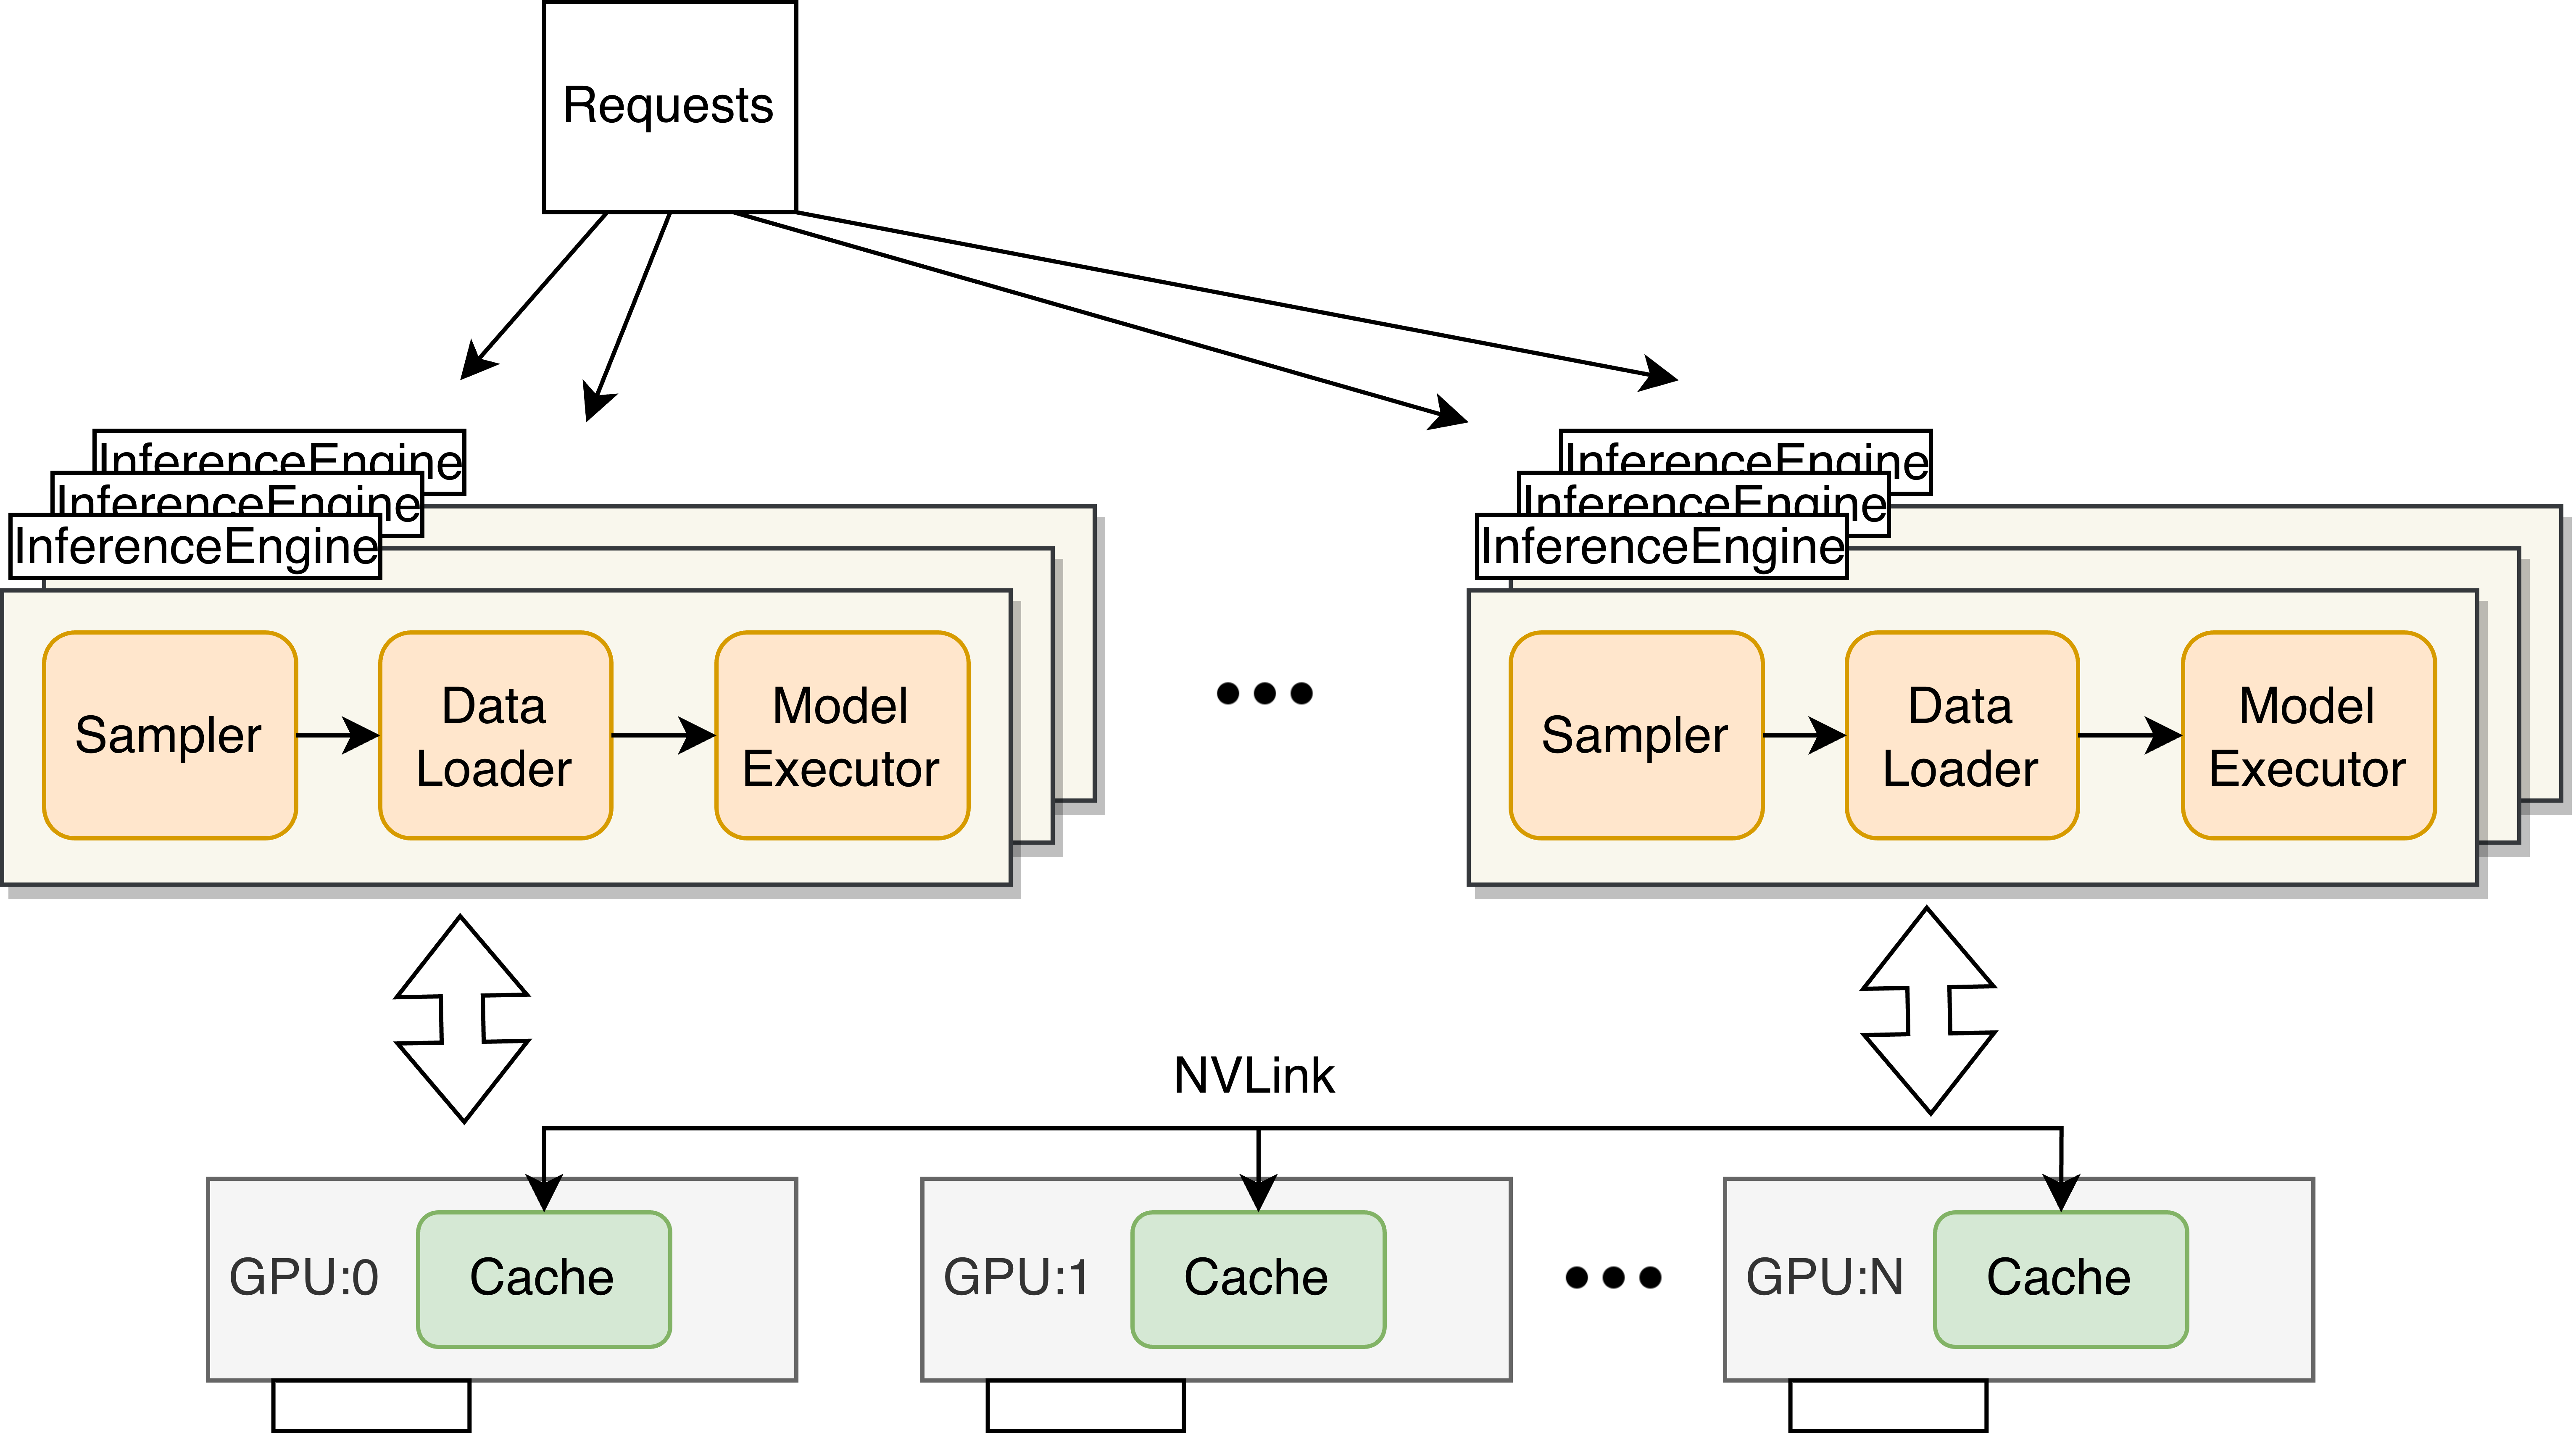
\includegraphics[width=\textwidth]{diagrams/group_meeting_gnn-System Diagram.png}
    
    \caption{System diagram}
    \label{Our system diagram}
\end{figure} 
\\ \\
\noindent \textbf{InferenceEngine Abstraction} \quad Due to Python's global interpreter lock, we leverage multiprocessing as the primary vehicle for inter-request concurrency. Our InferenceEngine abstraction represents a single process, which performs all operations for a single inference request - sampling, data loading, and model execution - sequentially. By binding InferenceEngines to a single GPU and containing these steps within a single process, we avoid any overheads due to IPC serialization. Multiple InferenceEngines can be created per GPU, which share GPU and host memory for resources such as model weights and graph features. All InferenceEngines share a request queue and response queue to receive inference requests and send back results. The InferenceEngine API supports any models or graph datasets that are built using DGL.
\\ \\ 
\noindent \textbf{Asynchronous Cache Update Thread Control} \quad Each InferenceEngine has a special C++ cache update thread linked using pybind11 \cite{pybind11} to perform cache update operations. Atomic integers required for masked cache updates are placed in shared memory using Boost \cite{BoostLibrary}. We also have one shared memory mutex per GPU to allow only one InferenceEngine's update thread to actively write at once. If the update thread fails to immediately acquire the lock, the update is skipped.
\\ \\
\noindent \textbf{GPU Sampling} \quad We use DGL's implementation of GPU sampling to perform the sampling stage. This requires graph structure (no features) to somehow be present in GPU memory. If graph structure can fit in a single GPU's memory, then the entire graph structure is copied to GPU memory during system initialization. If graph structure does not fit in GPU memory, we fall back to DGL's zero-copy functionality that allows GPUs to directly pull graph structure information from host memory when necessary \cite{PyTorch_Direct_2021}. 
\\ \\
\noindent \textbf{CUDA Multi-Process Serivce (MPS) \cite{CUDA_MPS}} \quad
To enable concurrent concurrent GPU kernel execution among InferenceEngines, we use NVIDIA CUDA MPS to provide a single CUDA context for all InferenceEngine processes. This is crucial for maximizing GPU utilization and avoiding unnecessary serialization of kernels, as many GPU kernels in our system do not fully occupy all SMs.

\section{Limitations}
Our system currently does not combine new inference requests into the existing graph or retrain the GNN to accommodate for new requests. 
Instead, we look only at GNN computation and investigate how to efficiently compute new embeddings. 
Integrating new nodes into the existing graph and dealing with challenges such as consistency are both orthogonal and out of scope of this work, but would be an interesting and natural extension.

  %%%%%%%%%%%%%%%%%%%%%%%%%%%%%%%%%%%%%%%%%%%%%%%%%%%%%%%%%%%%%%%%%%%%%%%%
\chapter{Evaluation} \label{Evaluation}
%%%%%%%%%%%%%%%%%%%%%%%%%%%%%%%%%%%%%%%%%%%%%%%%%%%%%%%%%%%%%%%%%%%%%%%%

%%%%%%%%%%%%%%%%%%%%%%%%%%%%%%%%%%%%%%%%%%%%%%%%%%%%%%%%%%%%%%%%%%%%%%%%
\section{Experimental Setup}
%%%%%%%%%%%%%%%%%%%%%%%%%%%%%%%%%%%%%%%%%%%%%%%%%%%%%%%%%%%%%%%%%%%%%%%%
\begin{enumerate}
    \item List all hardware, os, pytorch version, Dgl version
\end{enumerate}

\begin{enumerate}
    \item Data transfer size graphs also?
\end{enumerate}

\section{Datasets}

\begin{table}[h!]
    \begin{center}
        \begin{tabular}{|c c c c c|} 
        \hline
        \textbf{Dataset} & \textbf{Nodes} & \textbf{Edges} & \textbf{Features} & \textbf{Avg. Degree} \\ [0.5ex] 
        \hline\hline
        reddit & 200K & 111M & 602 & 492 \\
        \hline
        yelp & 700K & 13M & 500 & 10 \\
        \hline
        ogbn-products & 2.4M & 124M & 100 & 51.7 \\
        \hline
        ogbn-papers100M & 111M & 1.6B & 128 & 14.4 \\
        \hline
        \end{tabular}
    \end{center}
    % ogbn-products, uniform sampling, batch size 256, total latency 
    \caption{
        Information about graph datasets used in evaluation
    }
    \label{Eval: Dataset info}
\end{table}


%%%%%%%%%%%%%%%%%%%%%%%%%%%%%%%%%%%%%%%%%%%%%%%%%%%%%%%%%%%%%%%%%%%%%%%%
\section{Policy Evaluation}
%%%%%%%%%%%%%%%%%%%%%%%%%%%%%%%%%%%%%%%%%%%%%%%%%%%%%%%%%%%%%%%%%%%%%%%%

\subsection{Latency}
\begin{figure}[h!]
    \centering
    % 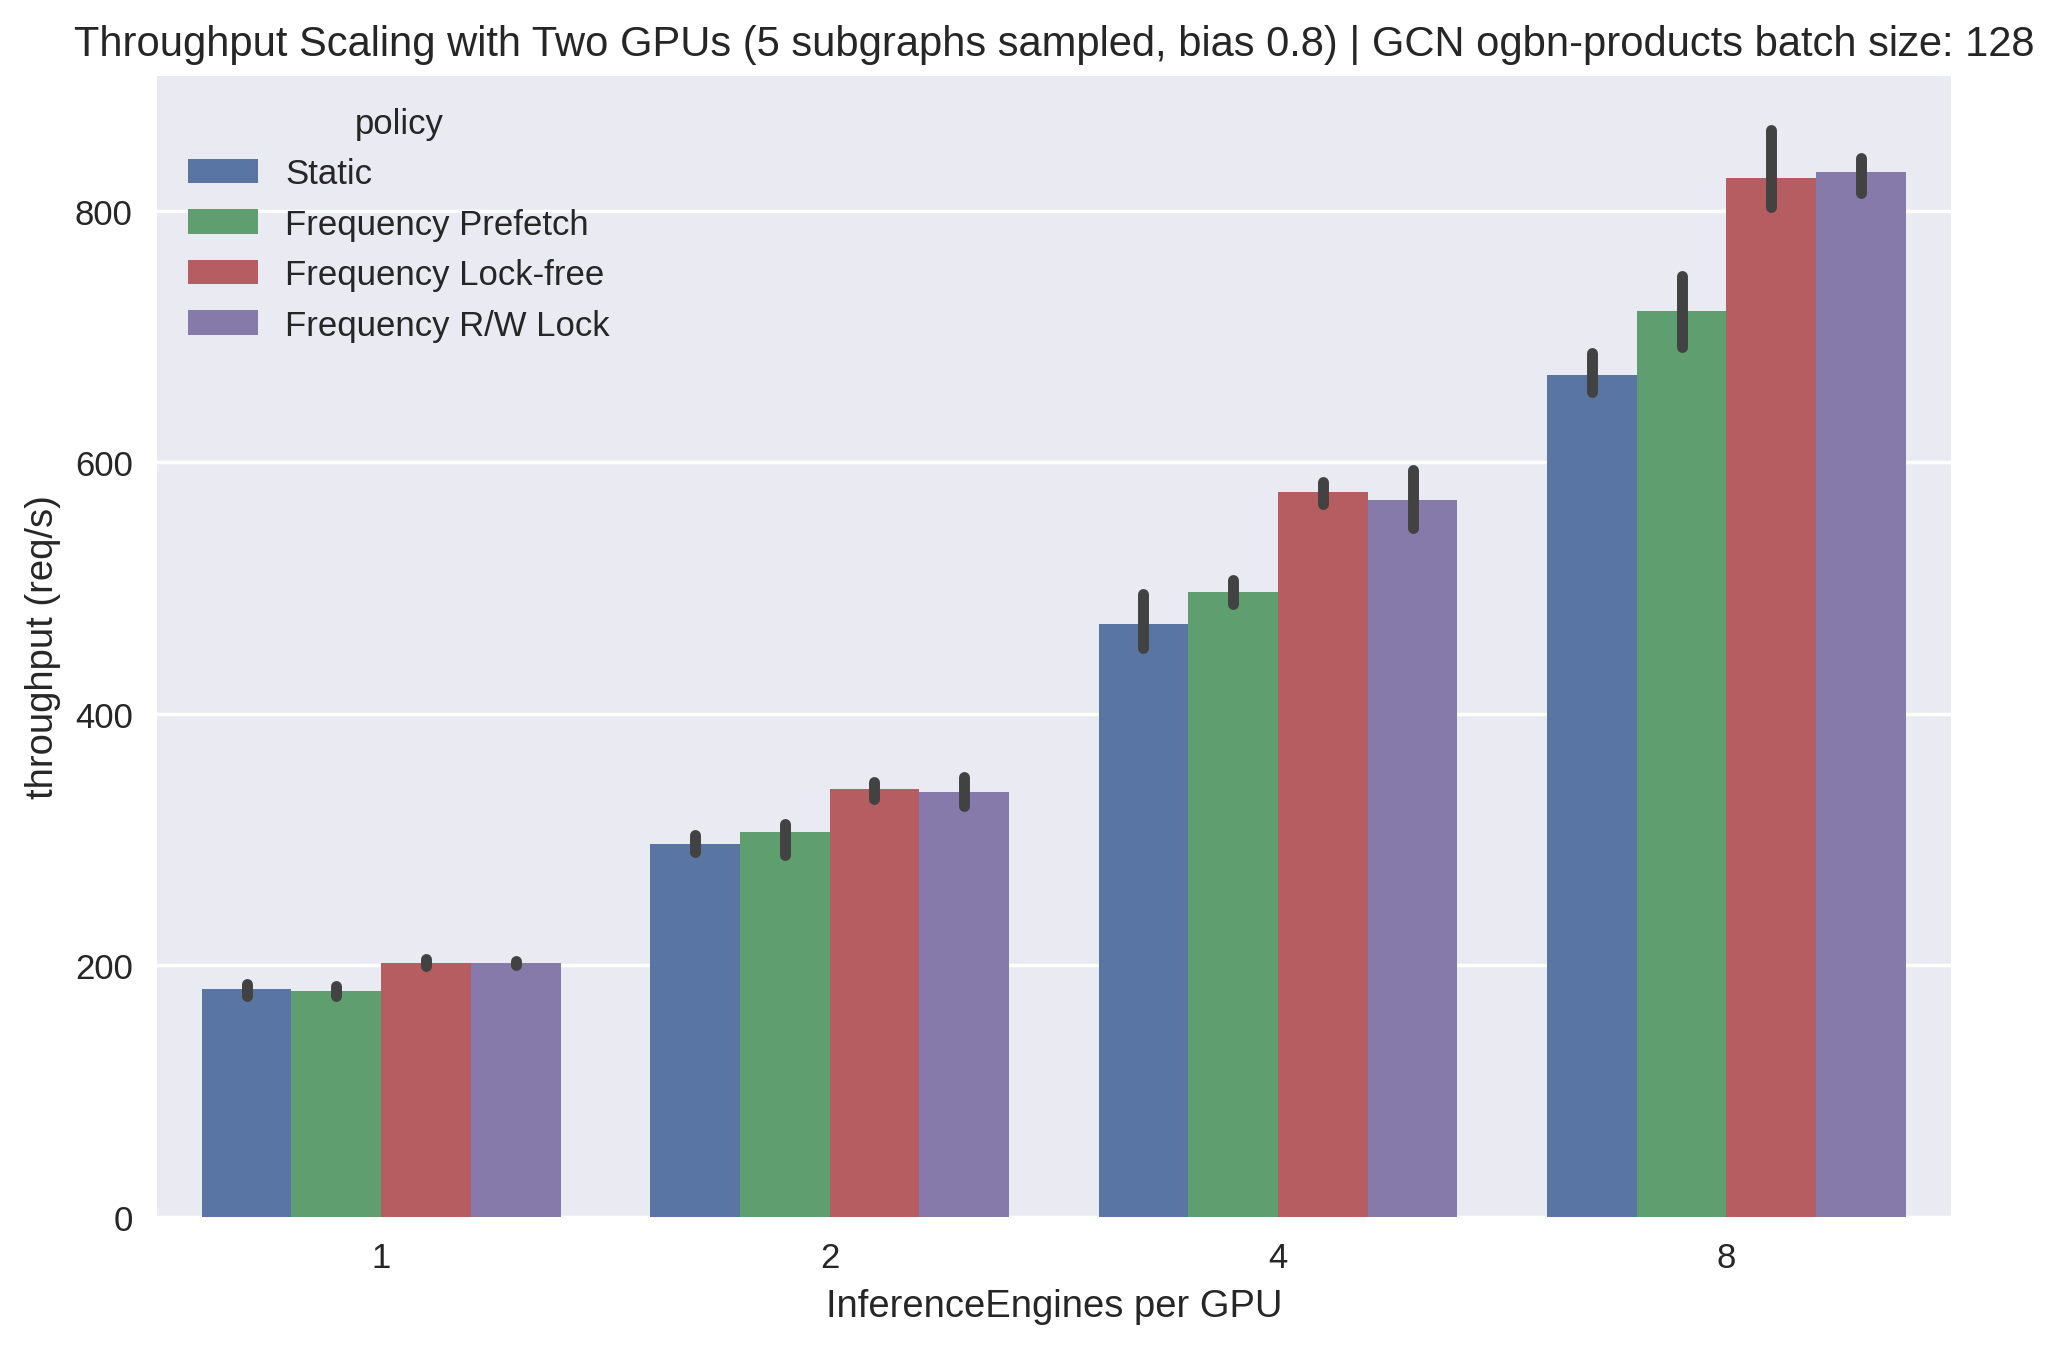
\includegraphics[width=\textwidth]{figures/throughput_GCN_bias_0.8_pinnedc0.2_gpus_2.png}
    \caption{[todo throughput]}
    \label{Eval: Latency speedup}
\end{figure}    

\subsection{Cache Hit Rate}
\begin{figure}[h!]
    \centering
    % 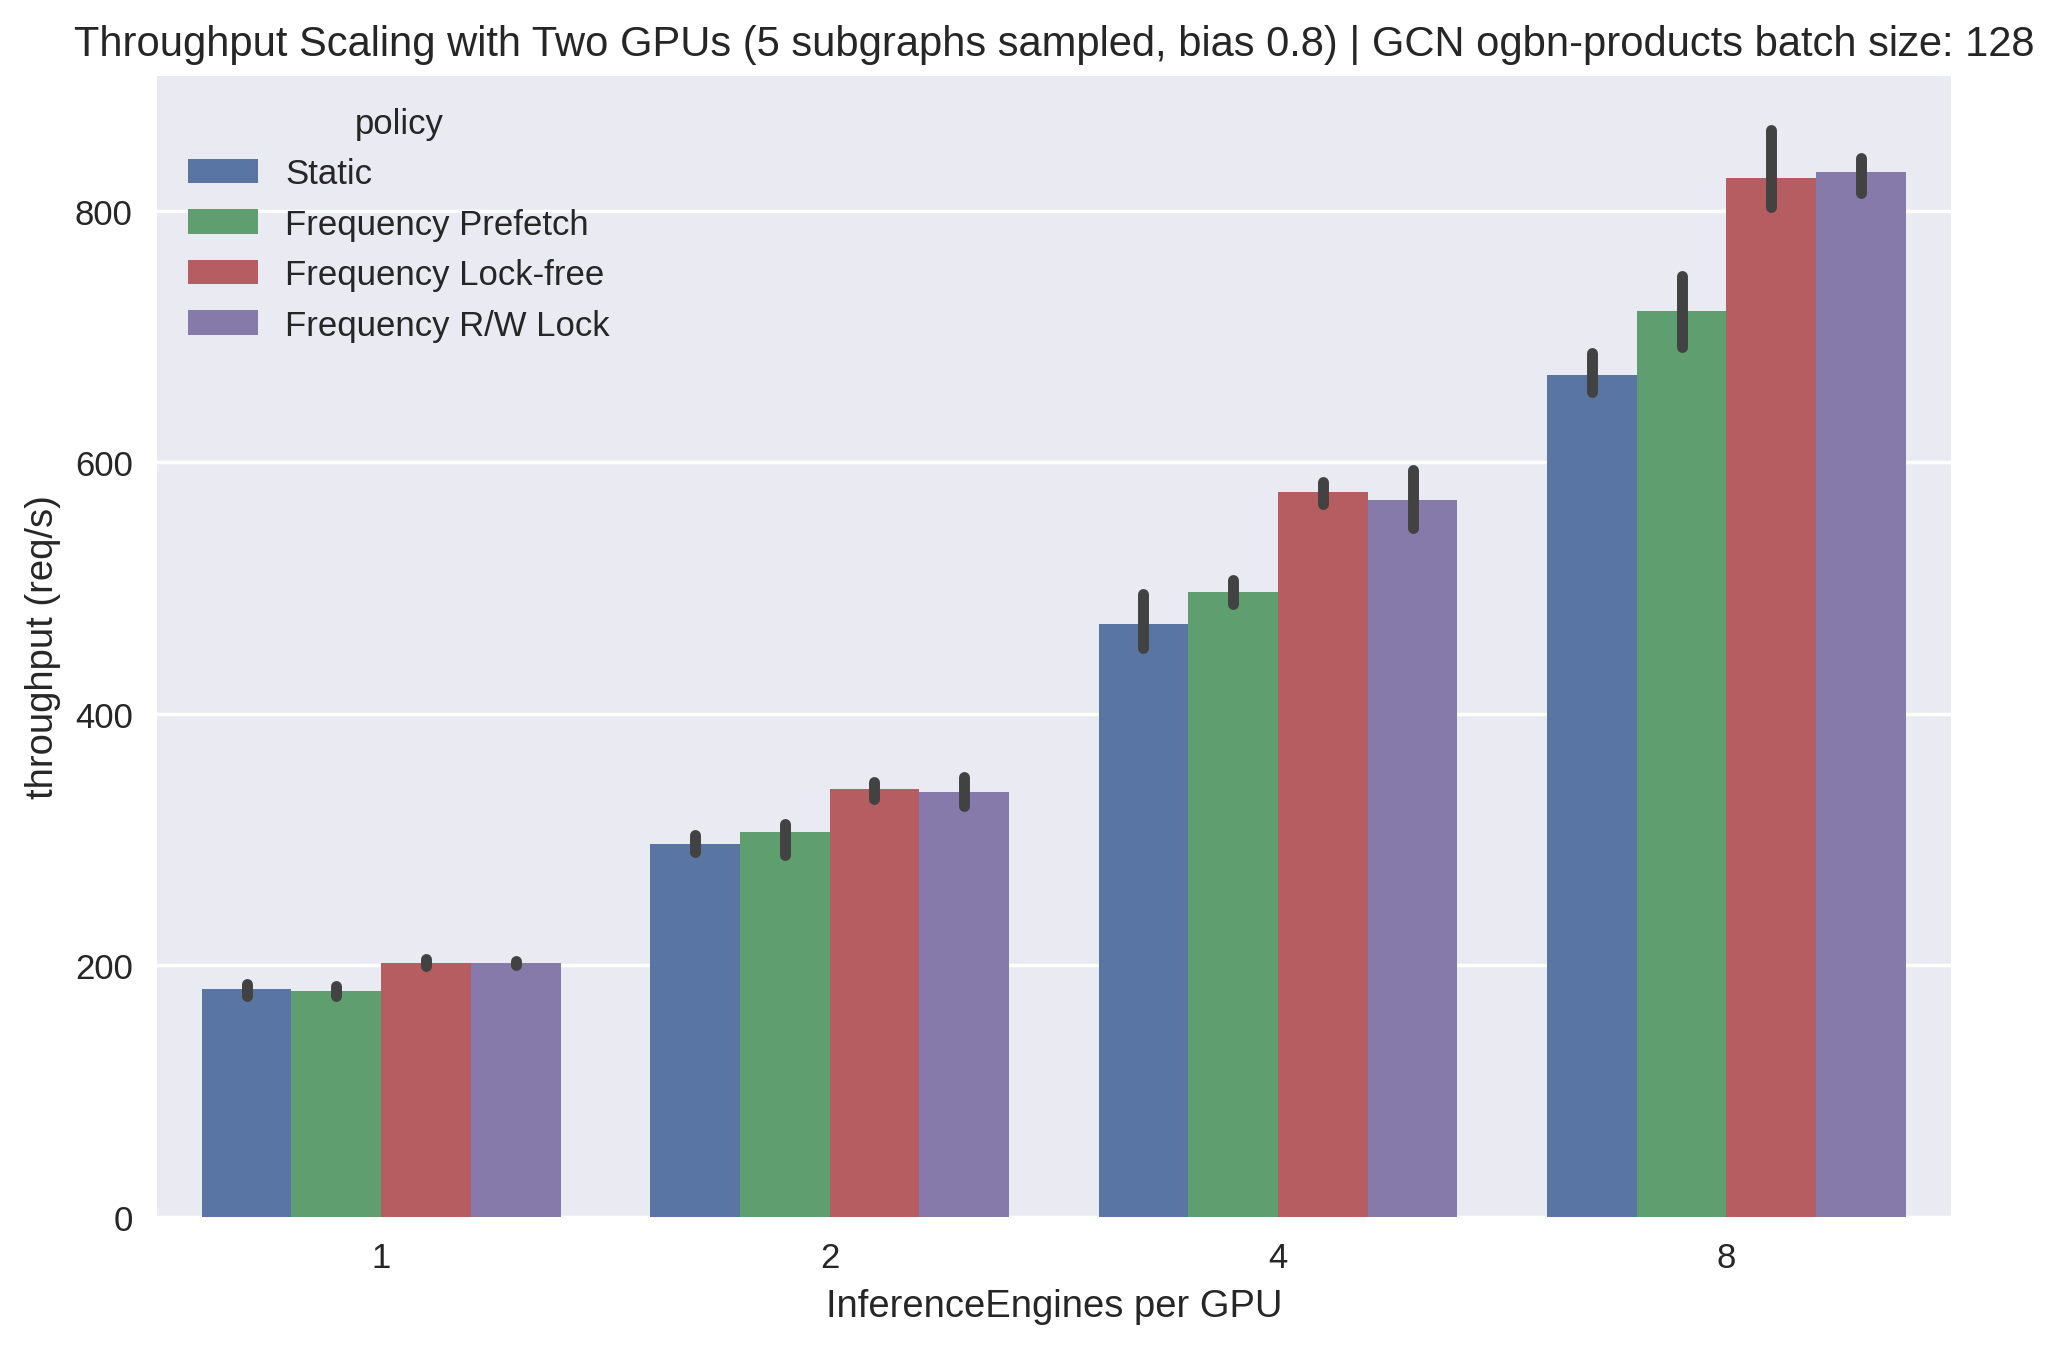
\includegraphics[width=\textwidth]{figures/throughput_GCN_bias_0.8_pinnedc0.2_gpus_2.png}
    \caption{[todo throughput]}
    \label{Eval: Hit Rate}
\end{figure}    
%%%%%%%%%%%%%%%%%%%%%%%%%%%%%%%%%%%%%%%%%%%%%%%%%%%%%%%%%%%%%%%%%%%%%%%%
\section{Locking vs. Lock-free}
%%%%%%%%%%%%%%%%%%%%%%%%%%%%%%%%%%%%%%%%%%%%%%%%%%%%%%%%%%%%%%%%%%%%%%%%

Figure \ref{Eval: Throughput} compares the throughput of our system using different cache replacement policies and mechanisms.

\subsection{Throughput}

\begin{figure}[h!]
    \centering
    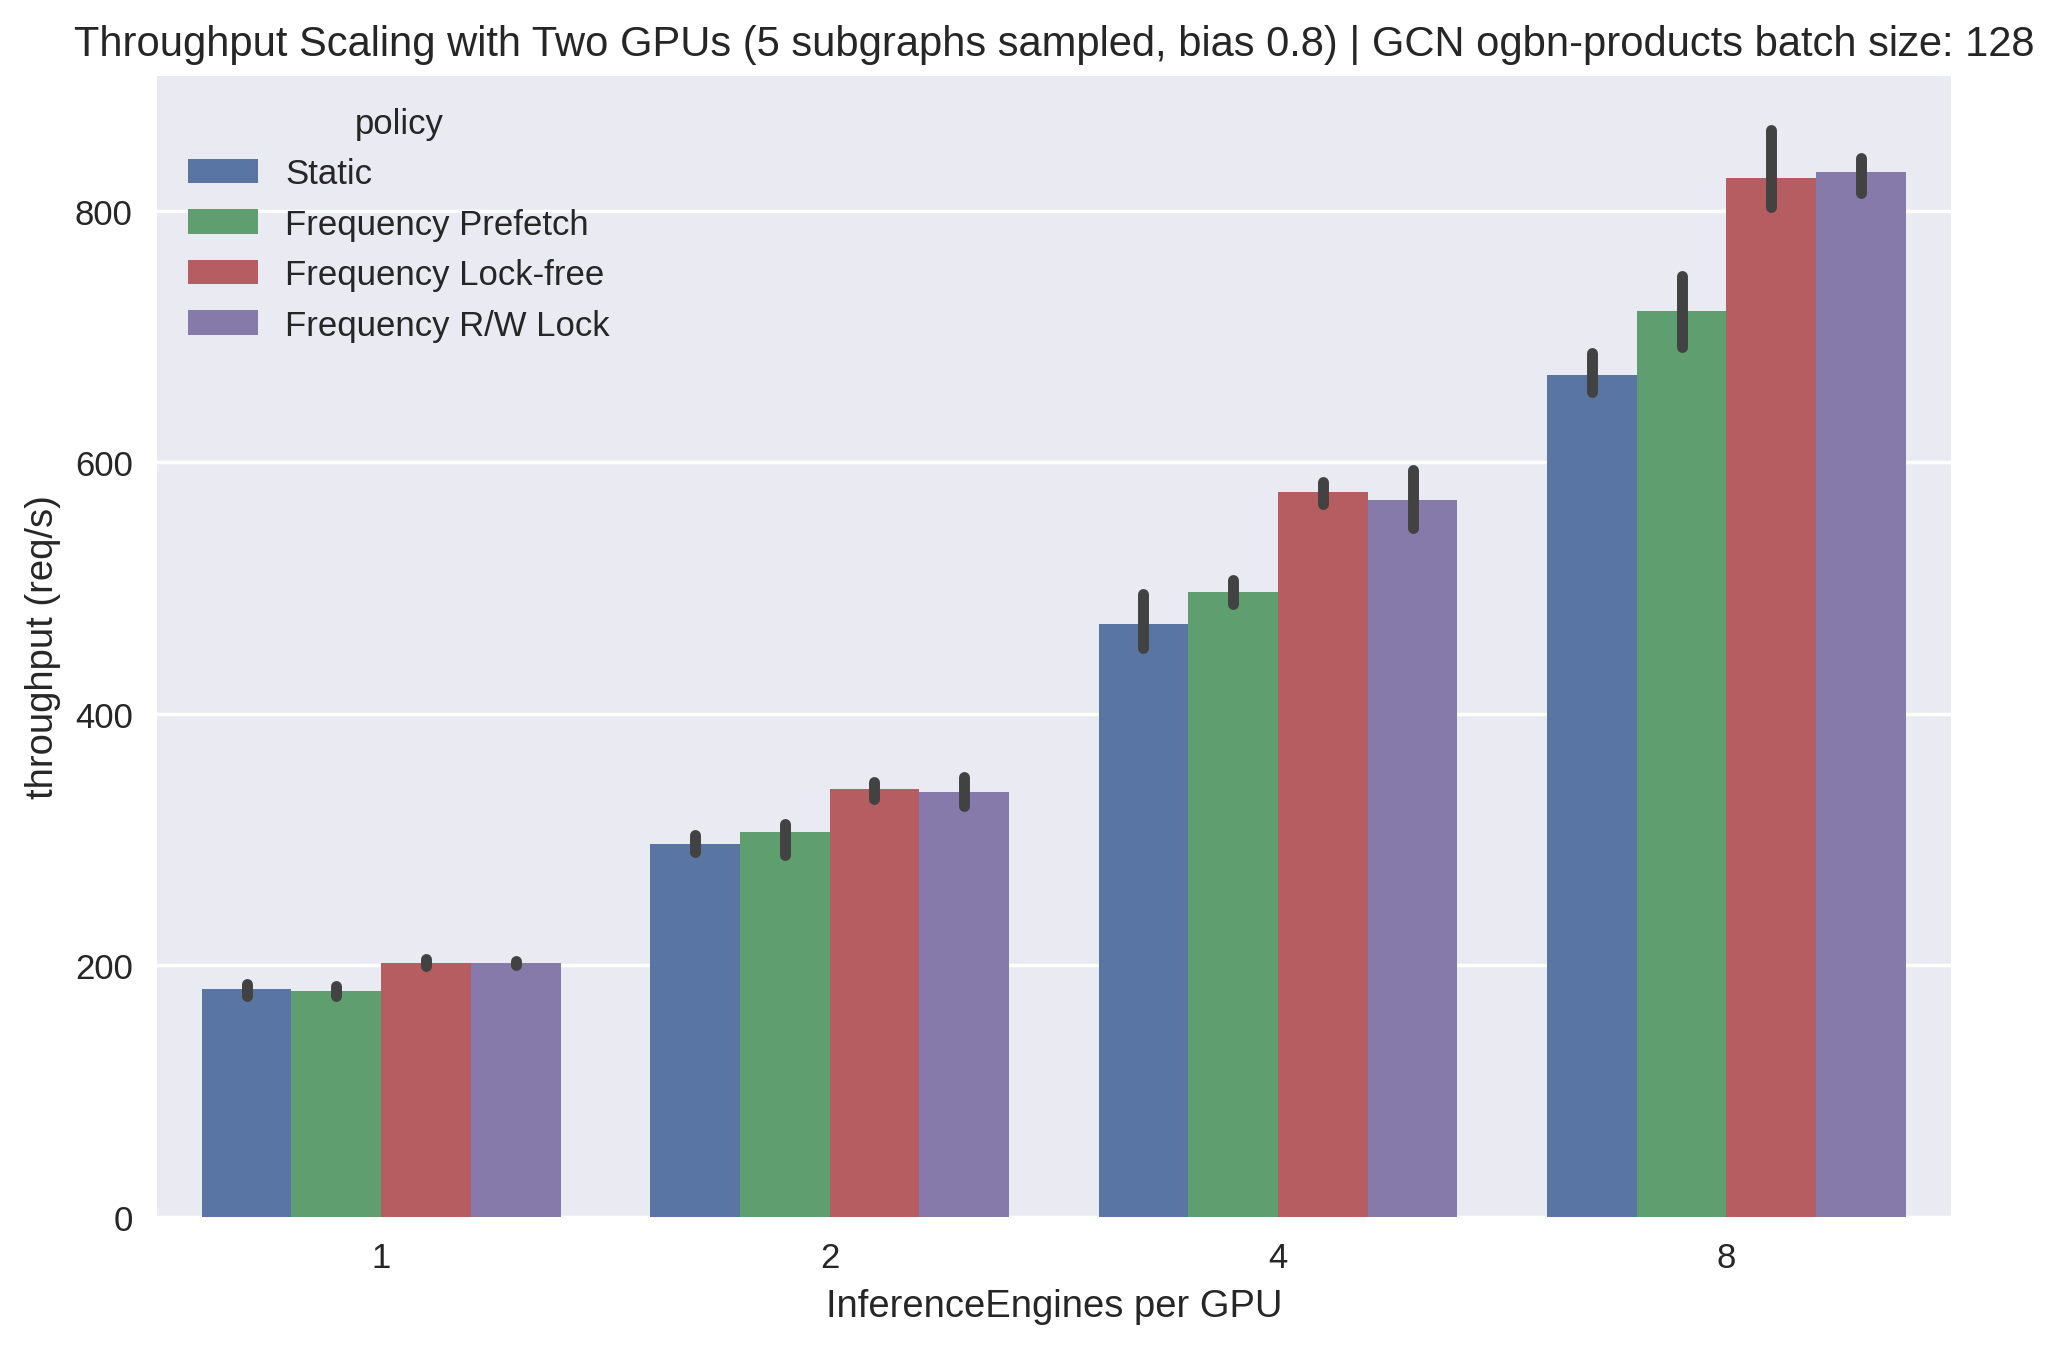
\includegraphics[width=0.8\textwidth]{figures/throughput_GCN_bias_0.8_pinnedc0.2_gpus_2.png}
    \caption{Peak throughput using two GPUs and varying number of InferenceEngines per GPU,}
    \label{Eval: Throughput}
\end{figure}    

Although there is little discernable difference in throughput between the lock-free and R/W lock approaches, there is an impact on P99 latency. Figure \ref{Eval: P99 latency} demonstrates these differences.
Note the log scale.

% \begin{figure}[h!]
%     \centering
%     % \includegraphics[width=\textwidth]{stamp_graphs.png}
    
%     \caption{[todo Lock conflict p99 latency]}
%     \label{Eval: P99 latency}
% \end{figure}    

To evaluate our system
\begin{figure}[h!]
    \centering
    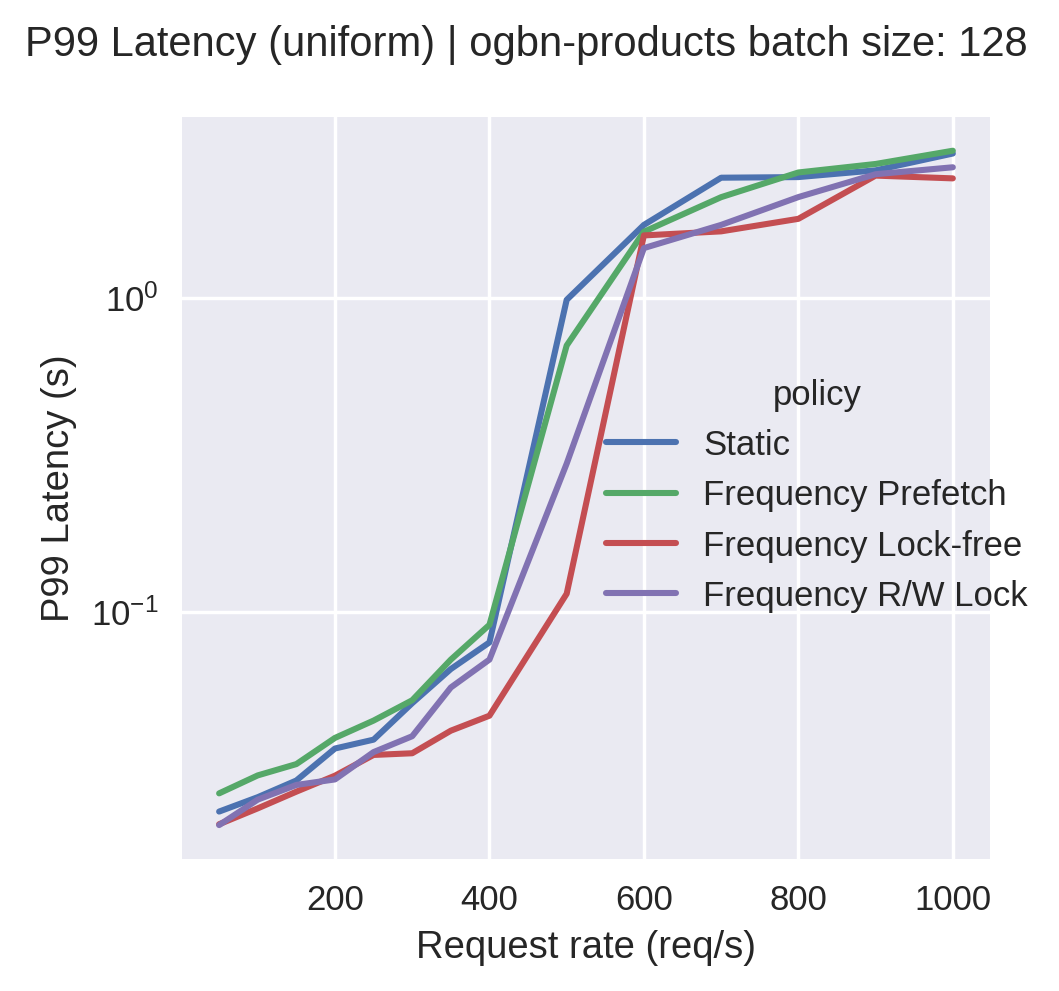
\includegraphics[width=0.85\textwidth]{figures/P99_latency_GCN_uniform_pinnedc0.2_gpus_3.png}    
    \caption{99\th percentile latencies for varying request rates. Tested on system using both GPUs and eight InferenceEngines per GPU.}
    \label{Eval: P99 latency}
\end{figure}  
Results are similar for the subgraph biased case.

\begin{figure}[h!]
    \centering
    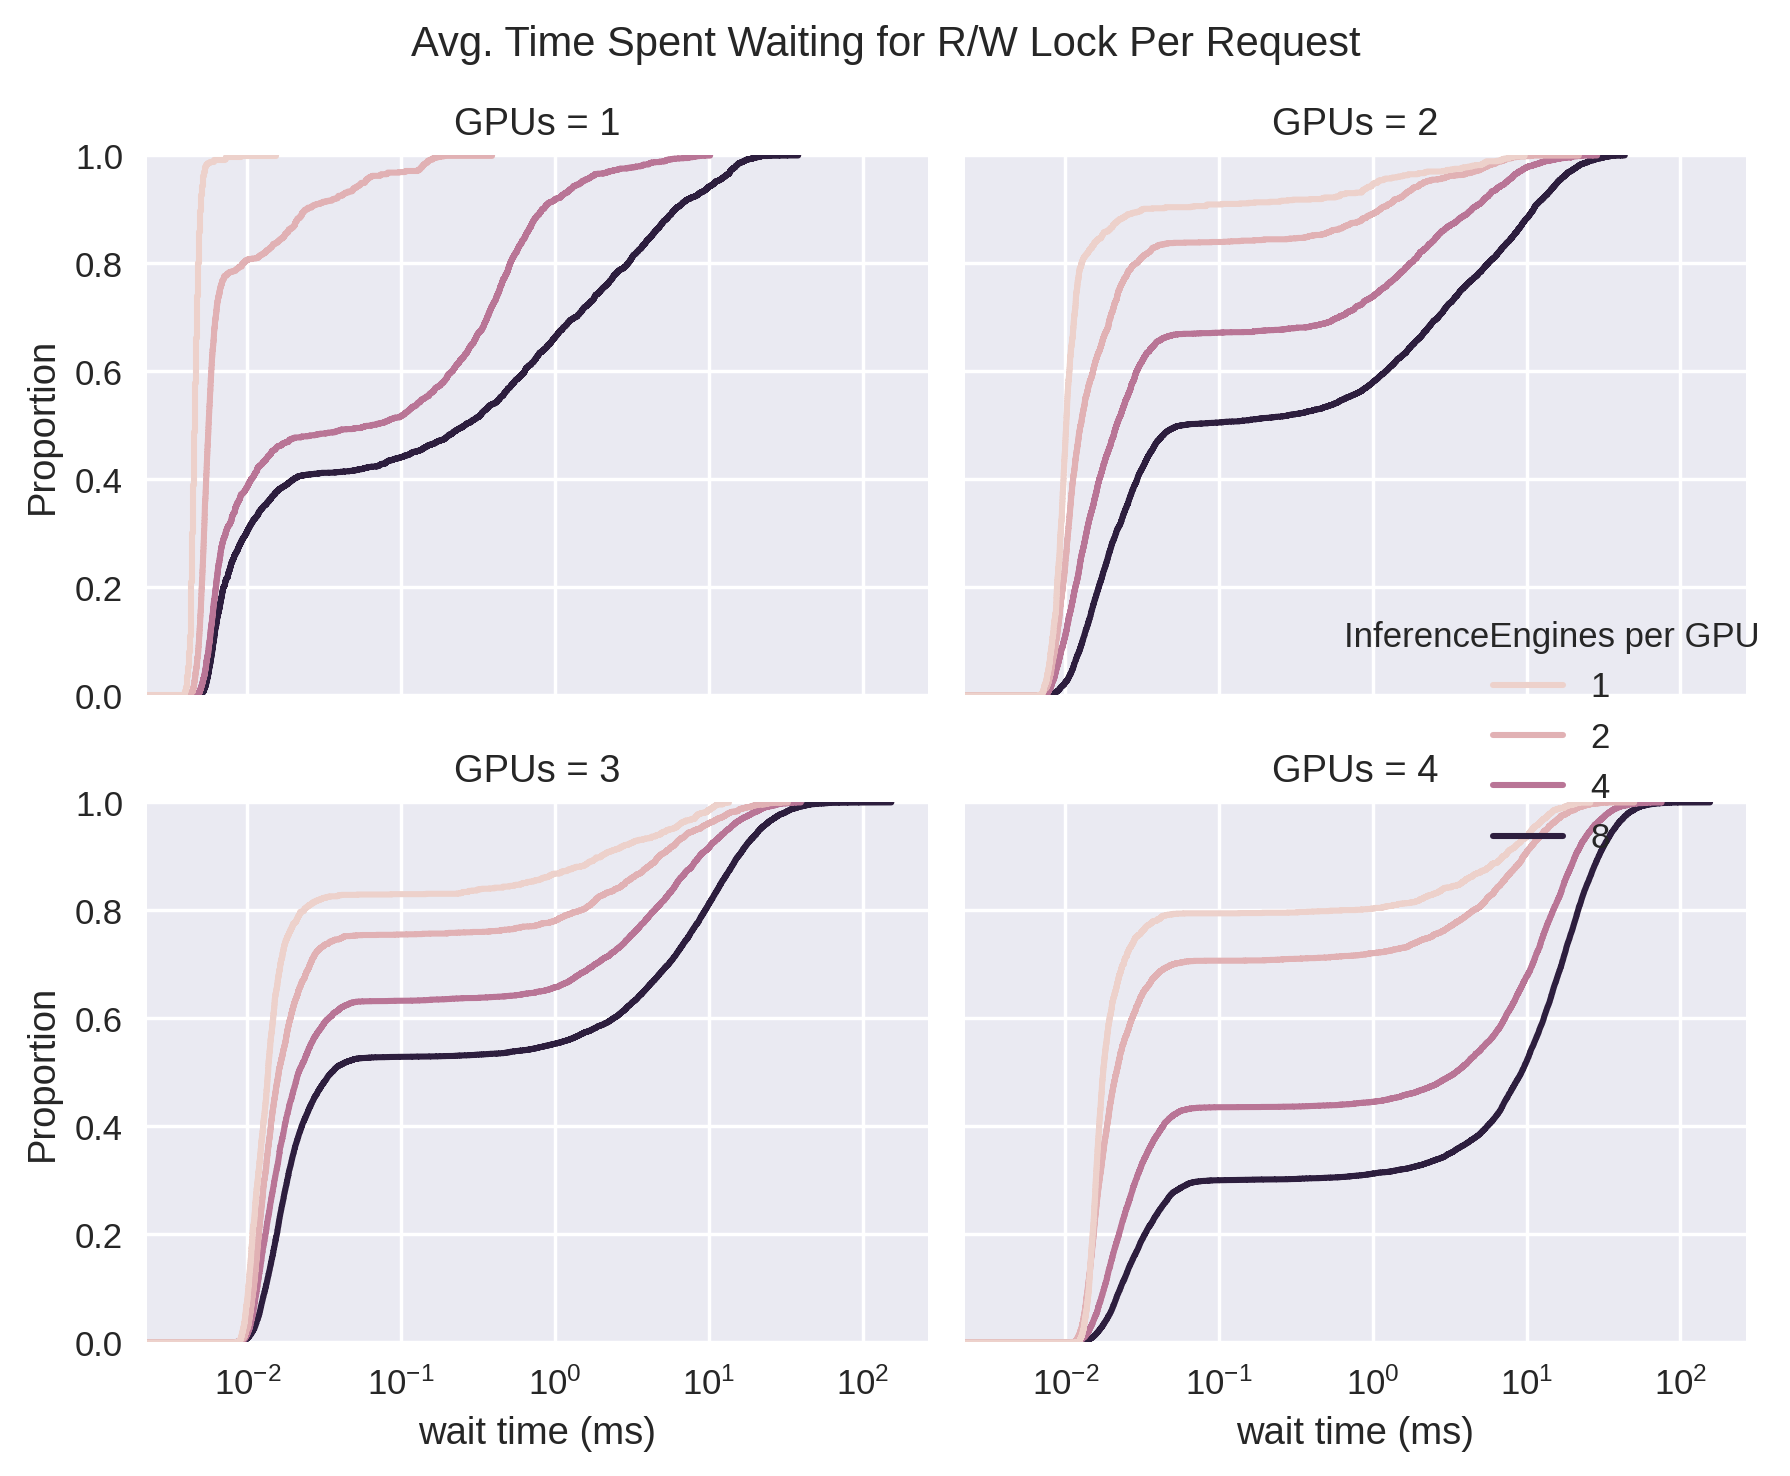
\includegraphics[width=\textwidth]{figures/Lock_Conflicts.png}
    
    \caption{[todo Lock conflict microbenchmark]}
    \label{Eval: Lock conflict microbenchmark}
\end{figure}    






%%%%%%%%%%%%%%%%%%%%%%%%%%%%%%%%%%%%%%%%%%%%%%%%%%%%%%%%%%%%%%%%%%%%%%%%
\section{PyTorch Direct Experiments}
%%%%%%%%%%%%%%%%%%%%%%%%%%%%%%%%%%%%%%%%%%%%%%%%%%%%%%%%%%%%%%%%%%%%%%%%

  %%%%%%%%%%%%%%%%%%%%%%%%%%%%%%%%%%%%%%%%%%%%%%%%%%%%%%%%%%%%%%%%%%%%%%%%
\chapter{Conclusion}
%%%%%%%%%%%%%%%%%%%%%%%%%%%%%%%%%%%%%%%%%%%%%%%%%%%%%%%%%%%%%%%%%%%%%%%%
  

% This ensures that the subsequent sections are being included as root
% items in the bookmark structure of your PDF reader.
\bookmarksetup{startatroot}
\backmatter

  % \begingroup
  %   \let\clearpage\relax
  %   \glsaddall
  %   % \printglossary[type=\acronymtype]
  %   % \newpage
  %   % \printglossary
  % \endgroup

  \printindex
  \printbibliography

\end{document}
